\documentclass{beamer}
%\usepackage{pgfpages}
% For 2 pages on 1
%\pgfpagesuselayout{2 on 1}[border shrink=2mm]
% For 4 pages on 1
%\pgfpagesuselayout{4 on 1}[border shrink=4mm]
%\usepackage{handoutWithNotes}
%\pgfpagesuselayout{3 on 1 with notes}[a4paper,border shrink=5mm]
\usepackage{graphicx}
\usepackage{amssymb}
\usepackage{amsmath}
\usepackage{multienum}
\usepackage{multicol}
\usepackage{enumitem}
\usepackage[super]{nth}
%\usepackage[margin=2cm]{geometry}
\usepackage{pgfplots}
\usepackage{fancyhdr}
\usepackage{units}
\usepackage{tikz}
\usepackage{filecontents}
\usetikzlibrary{arrows}
\usepackage{verbatim}
\usepackage{hyperref}
\hypersetup{pdfpagemode=FullScreen}

\usepackage{cancel}


\usepackage{animate}
\usepackage{tkz-fct}
\usepackage{color}

% These commands are being used in conjunction with the [handout] option in the document class declaration.
%\usepackage{pgfpages}
% For 2 pages on 1
%\pgfpagesuselayout{4 on 1}[border shrink=2mm]
% For 4 pages on 1
%\pgfpagesuselayout{4 on 1}[border shrink=2mm]
% A4 is a paper size used pretty much everywhere outside of the U.S. and Canada.
% We need to be more specific to use this paper size if we have installed a North American TeX distribution
%\pgfpagesuselayout{2 on 1}[a4paper, border shrink=5mm]
%\pgfpagesuselayout{4 on 1}[a4paper,landscape, border shrink=5mm]


\usetheme{Frankfurt}
\usecolortheme{orchid}
\usefonttheme{structurebold}

\title{The Definite Integral}
%\subtitle{MATH 252}
\author{Ryan Allison}
\institute{Eastern Washington University}
\date{December 16, 2013}
%\titlegraphic{\includegraphics[height=0.25\textheight]{mypup.jpg}}

\begin{document}

%=============Title=========
\begin{frame}
    \titlepage
\end{frame}


%===========First slide=========
%\section*{Outline}

\begin{frame}[t]
\frametitle{What is the Definite Integral?}

  	\begin{block}{Roughly speaking, the definite integral is the area between the curve and the $x$-axis on an interval $\left[a,b\right]$.}
 
	\begin{center}
 		\definecolor{ffqqqq}{rgb}{1,0,0}
		\definecolor{qqqqff}{rgb}{0,0,1}
		\begin{tikzpicture}[line cap=round,line join=round,>=triangle 45,x=1.0cm,y=1.0cm]
		\draw[->,color=black] (-1.7,0) -- (5.74,0);
		\foreach \x in {}
		\draw[shift={(\x,0)},color=black] (0pt,2pt) -- (0pt,-2pt) node[below] {\footnotesize $\x$};
		\draw[->,color=black] (0,-2.42) -- (0,2.12);
		\foreach \y in {}
		\draw[shift={(0,\y)},color=black] (2pt,0pt) -- (-2pt,0pt) node[left] {\footnotesize $\y$};
		\draw[color=black] (0pt,-10pt); %node[right] {\footnotesize $0$}
		\clip(-1.7,-2.42) rectangle (6,2.12);
		\draw[color=ffqqqq,fill=ffqqqq,fill opacity=0.1, smooth,samples=50,domain=0.0:2.0] plot(\x,{(-1)/5*\x*(\x-2)*(\x-5)}) -- (2,0) -- (0,0) -- cycle;
		\draw[color=qqqqff,fill=qqqqff,fill opacity=0.1, smooth,samples=50,domain=2.0:5.0] plot(\x,{(-1)/5*\x*(\x-2)*(\x-5)}) -- (5,0) -- (2,0) -- cycle;
		\draw[smooth,samples=100,domain=-1.7006859714273166:5.740703007864737] plot(\x,{(-1)/5*(\x)*((\x)-2)*((\x)-5)});
		\begin{scriptsize}
		\fill [color=qqqqff] (0,0) circle (1.5pt);
		\draw[color=qqqqff] (0.15,0.2) node {$a$};
		\fill [color=qqqqff] (5,0) circle (1.5pt);
		\draw[color=qqqqff] (5.05,0.2) node {$b$};
		\draw[color=black] (2.4, 1) node {$f(x)$};
		%\draw[color=qqqqff] (3.63,0.12) node {$b = 3.15$};
		
		\draw[color=black] (5.8, 0) node {$x$};
		\end{scriptsize}
		\end{tikzpicture}
		\end{center}
    \end{block}

    
\end{frame}

%==============Plane=========

\begin{frame}[plain]
Below is a graph of $v(t)$, the velocity (in $cm/s$) of an ice puck being pushed across a surface as a function of time (in sec).

    \frametitle{Why do we care about the area under the curve?} 

	\begin{columns}[t]
	    \column{0.6\textwidth}		
	    \begin{block}{$v(t)$}
	    	\definecolor{cqcqcq}{rgb}{0.75,0.75,0.75}
		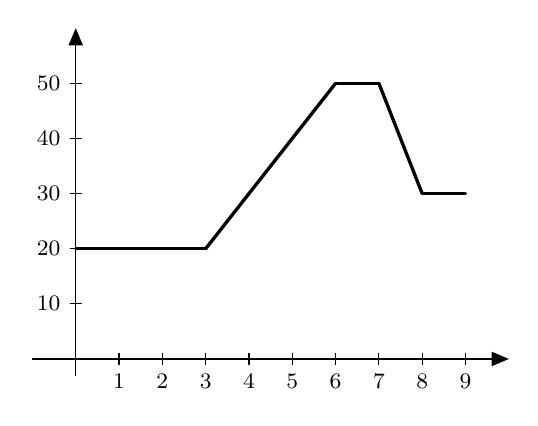
\begin{tikzpicture}[line cap=round,line join=round,>=triangle 45,x=.55cm,y=.07cm]
		%\draw [color=cqcqcq,dash pattern=on 17pt off 17pt, xstep=1.0cm,ystep=10.0cm] (-1,-3) grid (10,60);
		\draw[->,color=black] (-1,0) -- (10,0);
		\foreach \x in {1,2,3,4,5,6,7,8,9}
		\draw[shift={(\x,0)},color=black] (0pt,2pt) -- (0pt,-2pt) node[below] {\footnotesize $\x$};						\draw[->,color=black] (0,-3) -- (0,60);
		\foreach \y in {10,20,30,40,50}
		\draw[shift={(0,\y)},color=black] (2pt,0pt) -- (-2pt,0pt) node[left] {\footnotesize $\y$};
		%\draw[color=black] (0pt,-10pt) node[right] {\footnotesize $0$};
		\clip(-1,-3) rectangle (10,60);
		\draw[line width=1.2pt, smooth,samples=100,domain=0.0:3.0] plot(\x,{20});
		\draw[line width=1.2pt,smooth,samples=100,domain=3.0:6.0] plot(\x,{10*(\x)-10});
		\draw[line width=1.2pt,smooth,samples=100,domain=6.0:7.0] plot(\x,{50});
		\draw[line width=1.2pt,smooth,samples=100,domain=7.0:8.0] plot(\x,{0-20*(\x)+190});
		\draw[line width=1.2pt,smooth,samples=100,domain=8.0:9.0] plot(\x,{30});
		
		\end{tikzpicture}
			
			
			
			\end{block}
			\pause
	    \column{0.4\textwidth}
	    	\begin{block}{Question}
		
	 	\small{Calculate the area under the ``curve" on the interval $\left[0,9\right]$. What does this area tell us about the ice puck? }
		\end{block}
	    \end{columns}
\end{frame}  
    
    
 %==============Plane=========

\begin{frame}[plain]
\vspace{1pc}
Below is a graph of $v(t)$, the velocity (in $cm/s$) of an ice puck being pushed across a surface as a function of time (in sec).

\frametitle{Why do we care about the area under the curve?} 

	\begin{columns}[t]
	    \column{0.6\textwidth}		
	    \begin{block}{$v(t)$}
	    	\definecolor{zzttqq}{rgb}{0.6,0.2,0}
	    	\definecolor{cqcqcq}{rgb}{0.75,0.75,0.75}
		\begin{tikzpicture}[line cap=round,line join=round,>=triangle 45,x=.55cm,y=.07cm]
		%\draw [color=cqcqcq,dash pattern=on 17pt off 17pt, xstep=1.0cm,ystep=10.0cm] (-1,-3) grid (10,60);
		\draw[->,color=black] (-1,0) -- (10,0);
		\foreach \x in {1,2,3,4,5,6,7,8,9}
		\draw[shift={(\x,0)},color=black] (0pt,2pt) -- (0pt,-2pt) node[below] {\footnotesize $\x$};						
		\draw[->,color=black] (0,-3) -- (0,60);
		\foreach \y in {10,20,30,40,50}
		\draw[shift={(0,\y)},color=black] (2pt,0pt) -- (-2pt,0pt) node[left] {\footnotesize $\y$};
		%\draw[color=black] (0pt,-10pt) node[right] {\footnotesize $0$};
		\clip(-1,-3) rectangle (10,60);
\draw[line width=0pt,color=zzttqq,fill=zzttqq, opacity=0.1, smooth,samples=50,domain=3.0:6.0] plot(\x,{10*\x-10}) -- (6,0) -- (3,0) -- cycle;
\draw[line width=0pt,color=zzttqq,fill=zzttqq, opacity=0.1, smooth,samples=50,domain=6.0:7.0] plot(\x,{50}) -- (7,0) -- (6,0) -- cycle;
\draw[line width=0pt,color=zzttqq,fill=zzttqq, opacity=0.1, smooth,samples=50,domain=7.0:8.0] plot(\x,{0-20*\x+190}) -- (8,0) -- (7,0) -- cycle;
\draw[line width=0pt,color=zzttqq,fill=zzttqq, opacity=0.1, smooth,samples=50,domain=8.0:9.0] plot(\x,{30}) -- (9,0) -- (8,0) -- cycle;
\draw[line width=0pt,color=zzttqq,fill=zzttqq, opacity=0.1, smooth,samples=50,domain=0.0:3.0] plot(\x,{20}) -- (3,0) -- (0,0) -- cycle;
		\draw[line width=1.2pt, smooth,samples=100,domain=0.0:3.0] plot(\x,{20});
		\draw[line width=1.2pt,smooth,samples=100,domain=3.0:6.0] plot(\x,{10*(\x)-10});
		\draw[line width=1.2pt,smooth,samples=100,domain=6.0:7.0] plot(\x,{50});
		\draw[line width=1.2pt,smooth,samples=100,domain=7.0:8.0] plot(\x,{0-20*(\x)+190});
		\draw[line width=1.2pt,smooth,samples=100,domain=8.0:9.0] plot(\x,{30});
		%\draw [line width=.4pt,dash pattern=on 4pt off 4pt,color=black] (3,0)-- (3,20);
		\draw [line width=.4pt,dash pattern=on 4pt off 4pt,color=black] (6,20)-- (6,50);
		\draw [line width=.4pt,dash pattern=on 4pt off 4pt,color=black] (7,30)-- (7,50);
		\draw [line width=.4pt,dash pattern=on 4pt off 4pt,color=black] (9,0)-- (9,30);
		\draw [line width=.4pt,dash pattern=on 4pt off 4pt,color=black] (3,20)-- (9,20);
		\draw [line width=.4pt,dash pattern=on 4pt off 4pt,color=black] (6,30)-- (8,30);
		\draw (3.5,13) node[anchor=north west] {$A_1$};
		\draw (4, 28) node[anchor=north west] {$A_2$};
		\draw (6, 43) node[anchor=north west] {$A_3$};
		\draw (6.8, 37) node[anchor=north west] {$A_4$};
		\draw (7,28) node[anchor=north west] {$A_5$};
		\end{tikzpicture}
			\end{block}
	    \column{0.2\textwidth}
	  
	   		 \begin{align*}
   				A &=\sum_{i=1}^{5}A_i \\
					&=A_1 + A_2 + A_3 + A_4 + A_5\\
					&= \left(180 + 45 + 20 + 10 + 30\right) \\
					&= 285\left(\dfrac{sec}{1} \cdot \dfrac{cm}{sec}\right) \\
					&= 285\left(\dfrac{\cancel{sec}}{1} \cdot \dfrac{cm}{\cancel{sec}}\right) \\
					&= 285 cm
			\end{align*} 
		
	    \end{columns}
	    
	    %\vspace{1pc}
															%Fix spacing	   


\end{frame}  

 %==============Plane=========

\begin{frame}[plain]
\vspace{1pc}
Below is a graph of $v(t)$, the velocity (in $cm/s$) of an ice puck being pushed across a surface as a function of time (in sec).

\frametitle{Why do we care about the area under the curve?} 

	\begin{columns}[t]
	    \column{0.6\textwidth}		
	    \begin{block}{$v(t)$}
	    	\definecolor{zzttqq}{rgb}{0.6,0.2,0}
	    	\definecolor{cqcqcq}{rgb}{0.75,0.75,0.75}
		\begin{tikzpicture}[line cap=round,line join=round,>=triangle 45,x=.55cm,y=.07cm]
		%\draw [color=cqcqcq,dash pattern=on 17pt off 17pt, xstep=1.0cm,ystep=10.0cm] (-1,-3) grid (10,60);
		\draw[->,color=black] (-1,0) -- (10,0);
		\foreach \x in {1,2,3,4,5,6,7,8,9}
		\draw[shift={(\x,0)},color=black] (0pt,2pt) -- (0pt,-2pt) node[below] {\footnotesize $\x$};						
		\draw[->,color=black] (0,-3) -- (0,60);
		\foreach \y in {10,20,30,40,50}
		\draw[shift={(0,\y)},color=black] (2pt,0pt) -- (-2pt,0pt) node[left] {\footnotesize $\y$};
		%\draw[color=black] (0pt,-10pt) node[right] {\footnotesize $0$};
		\clip(-1,-3) rectangle (10,60);
\draw[line width=0pt,color=zzttqq,fill=zzttqq, opacity=0.1, smooth,samples=50,domain=3.0:6.0] plot(\x,{10*\x-10}) -- (6,0) -- (3,0) -- cycle;
\draw[line width=0pt,color=zzttqq,fill=zzttqq, opacity=0.1, smooth,samples=50,domain=6.0:7.0] plot(\x,{50}) -- (7,0) -- (6,0) -- cycle;
\draw[line width=0pt,color=zzttqq,fill=zzttqq, opacity=0.1, smooth,samples=50,domain=7.0:8.0] plot(\x,{0-20*\x+190}) -- (8,0) -- (7,0) -- cycle;
\draw[line width=0pt,color=zzttqq,fill=zzttqq, opacity=0.1, smooth,samples=50,domain=8.0:9.0] plot(\x,{30}) -- (9,0) -- (8,0) -- cycle;
\draw[line width=0pt,color=zzttqq,fill=zzttqq, opacity=0.1, smooth,samples=50,domain=0.0:3.0] plot(\x,{20}) -- (3,0) -- (0,0) -- cycle;
		\draw[line width=1.2pt, smooth,samples=100,domain=0.0:3.0] plot(\x,{20});
		\draw[line width=1.2pt,smooth,samples=100,domain=3.0:6.0] plot(\x,{10*(\x)-10});
		\draw[line width=1.2pt,smooth,samples=100,domain=6.0:7.0] plot(\x,{50});
		\draw[line width=1.2pt,smooth,samples=100,domain=7.0:8.0] plot(\x,{0-20*(\x)+190});
		\draw[line width=1.2pt,smooth,samples=100,domain=8.0:9.0] plot(\x,{30});
		%\draw [line width=.4pt,dash pattern=on 4pt off 4pt,color=black] (3,0)-- (3,20);
		\draw [line width=.4pt,dash pattern=on 4pt off 4pt,color=black] (6,20)-- (6,50);
		\draw [line width=.4pt,dash pattern=on 4pt off 4pt,color=black] (7,30)-- (7,50);
		\draw [line width=.4pt,dash pattern=on 4pt off 4pt,color=black] (9,0)-- (9,30);
		\draw [line width=.4pt,dash pattern=on 4pt off 4pt,color=black] (3,20)-- (9,20);
		\draw [line width=.4pt,dash pattern=on 4pt off 4pt,color=black] (6,30)-- (8,30);
		\draw (3.5,13) node[anchor=north west] {$A_1$};
		\draw (4, 28) node[anchor=north west] {$A_2$};
		\draw (6, 43) node[anchor=north west] {$A_3$};
		\draw (6.8, 37) node[anchor=north west] {$A_4$};
		\draw (7,28) node[anchor=north west] {$A_5$};
		\end{tikzpicture}
			\end{block}
	    \column{0.4\textwidth}
	    \begin{block}{Question}
	 	\small{Calculate the area under the ``curve" on the interval $\left[0,9\right]$. What does this area tell us about the ice puck? }
	    \end{block}
	    \pause
	    \begin{block}{Answer}
	    The puck traveled a total distance of 285 cm in \\ 9 seconds. 
	    \end{block}
	    \end{columns}
	    
	    %\vspace{1pc}
															%Fix spacing	   


\end{frame}  

%===========Triangle=========
%\begin{frame}[plain]
%\frametitle{Why do we care about the area under the curve?} 
	
%The graph shows the function, $g$, that models a bicyclist's velocity in feet per second, over time, $t$, in seconds.

%    \begin{columns}[t]
%	    \column{0.6\textwidth}				
%	    \begin{block}{$y=g(t)$}
%		\begin{tikzpicture}[line cap=round,line join=round,>=triangle 45,x=.757cm,y=.1cm]
%			\draw[->,color=black] (-0.5,0) -- (7,0);
%			\foreach \x in {1,2,3,4,5,6}
%			\draw[shift={(\x,0)},color=black] (0pt,2pt) -- (0pt,-2pt) node[below] {\footnotesize $\x$};
%			\draw[->,color=black] (0,-1) -- (0,23);
%			\foreach \y in {5,10,15,20}
%			\draw[shift={(0,\y)},color=black] (2pt,0pt) -- (-2pt,0pt) node[left] {\footnotesize $\y$};
			%\draw[color=black] (0pt,-10pt) node[right] {};
%			\clip(-1,-6) rectangle (8,21);
%			\draw[line width=1.2pt, smooth,samples=100,domain=0.0:6.0] plot(\x,{(-20)/3*abs((\x)-3)+20});
			%\draw[color=black] (5,12) node{$g(t)$};
%			\draw[color=black] (7,-3) node{$t$};
%		\end{tikzpicture}
%	      \end{block}	

%	  \column{0.4\textwidth}
%	   \end{columns}
%	   \vspace{2pc}
%\end{frame}

%============Triangle=========
%\begin{frame}[plain]
%\frametitle{Why do we care about the area under the curve?} 
% \vspace{1pc}
%What does the area under the curve from [0,6] tell us about the biker?
 
%   \begin{columns}[t]
  
%	\column{0.6\textwidth}
%	\begin{block}{$y=g(t)$}			
%			\definecolor{wwqqcc}{rgb}{0.4,0,0.8}
%			\definecolor{ffqqtt}{rgb}{1,0,0.2}
%	\begin{tikzpicture}[line cap=round,line join=round,>=triangle 45,x=.757cm,y=.1cm]
%		\draw[->,color=black] (-0.5,0) -- (7,0);
%		\foreach \x in {1,2,3,4,5,6}
%		\draw[shift={(\x,0)},color=black] (0pt,2pt) -- (0pt,-2pt) node[below] {\footnotesize $\x$};
%		\draw[->,color=black] (0,-1) -- (0,23);
%		\foreach \y in {5,10,15,20}
%		\draw[shift={(0,\y)},color=black] (2pt,0pt) -- (-2pt,0pt) node[left] {\footnotesize $\y$};
%		\draw[color=black] (0pt,-10pt) node[right] {};
%		\clip(-1,-6) rectangle (8,21);
%		\draw[color=ffqqtt,fill=ffqqtt,fill opacity=0.1, smooth,samples=50,domain=0.0:6.0] plot(\x,{(-20)/						3*abs(\x-3)+20}) -- (6,0) -- (0,0) -- cycle;
%		\draw[line width=1.2pt, smooth,samples=100,domain=0.0:6.0] plot(\x,{(-20)/3*abs((\x)-3)+20});
%		\draw [line width=1.2pt,dash pattern=on 4pt off 4pt,color=wwqqcc] (3,19.8)-- (3,0);
%		\draw[color=black] (7,-3) node{$t$};
%		\begin{scriptsize}
%			\draw[color=wwqqcc] (2.7,10) node {$h$};
%		\end{scriptsize}
%	\end{tikzpicture}\pause\\
%	\end{block}
	
	
%      \column{0.4\textwidth}
      %\begin{block}												%FIX Not working!
%      		\begin{align*}
   %			A &=\dfrac{1}{2} \cdot (b) \cdot (h) \\
%    				&=\dfrac{1}{2} \cdot (6 sec) \cdot \left(20 \dfrac{ft}{sec}\right)\\
%				&=\left(\dfrac{1}{2} \cdot 6 \cdot 20\right) \cdot \left(\dfrac{sec}{1}\cdot \dfrac{ft}{sec}\right)\\	
%				&=\left(3 \cdot 20\right) \cdot \left(\dfrac{\cancel{sec}}{1}\cdot \dfrac{ft}{\cancel{sec}}\right)\\	
%				&= 60 ft 
%		\end{align*} 
      %\end{block}
			
%	   \end{columns} 
%	   \pause 
	   
%	   \vspace{1pc}
															%Fix spacing	   

%\bf{The area under the curve tells us how far the biker traveled.} 
% \end{frame} 
    


%==============Primary1=========
\begin{frame}[plain] 
\frametitle{How would we find the area under this curve?} 
 
 \begin{columns}
 	\column{0.6\textwidth}	
	\begin{block}{$y=f(x)$}
 			\definecolor{zzwwqq}{rgb}{0.6,0.4,0}
			\definecolor{xdxdff}{rgb}{0.49,0.49,1}
			\definecolor{zzttqq}{rgb}{0.6,0.2,0}
			\begin{tikzpicture}[line cap=round,line join=round,>=triangle 45,x=.7cm,y=.7cm]
			\draw[->,color=black] (-1,0) -- (8,0);
			\foreach \x in {-1,1,2,3,4,5,6,7}
			\draw[shift={(\x,0)},color=black] (0pt,2pt) -- (0pt,-2pt);
			\draw[->,color=black] (0,-1) -- (0,8);
			\foreach \y in {,1,2,3,4,5,6,7}
			\draw[shift={(0,\y)},color=black] (2pt,0pt) -- (-2pt,0pt);
			\clip(-1,-1) rectangle (8,8);
			\draw[color=zzwwqq,fill=zzwwqq,fill opacity=0.1,smooth,samples=50,domain=0.9968591090975547:6.0] plot(\x,{(3/2)^(\x-1)}) -- (6,0) -- (1,0) -- cycle;
			\draw[line width=1.2pt, smooth,samples=100,domain=1.0:6.0] plot(\x,{(3/2)^((\x)-1)});
			\begin{scriptsize}	
			\fill [color=xdxdff] (1,0) circle (1.5pt);
			\draw[color=xdxdff] (1.12,0.21) node {$a$};
			\fill [color=xdxdff] (6,0) circle (1.5pt);
			\draw[color=xdxdff] (6.11,0.21) node {$b$};
			%\draw[color=zzttqq] (3.97,1.54) node {$Area = 19.27$};
			\draw[color=black] (2.5,6) node {$Area = 16.27$};
			\end{scriptsize}
			\end{tikzpicture}
	\end{block}	
\column{0.4\textwidth} 
 \end{columns}
\end{frame}


%==============Delta_X=========
\begin{frame} [plain]
\frametitle{How would we find the area under this curve?} 
 %First let's try cutting the interval into a finite number of pieces. 
\begin{columns}[t]
		\column{0.6\textwidth}	
		\begin{block}{$y=f(x)$}
 				\definecolor{zzwwqq}{rgb}{0.6,0.4,0}
				\definecolor{zzttqq}{rgb}{0.6,0.2,0}
				\definecolor{xdxdff}{rgb}{0.49,0.49,1}
				\begin{tikzpicture}[line cap=round,line join=round,>=triangle 45,x=.7cm,y=.7cm]
				\draw[->,color=black] (-1,0) -- (8,0);
				\foreach \x in {-1,1,2,3,4,5,6,7}
				\draw[shift={(\x,0)},color=black] (0pt,2pt) -- (0pt,-2pt);
				\draw[->,color=black] (0,-1) -- (0,8);
				\foreach \y in {,1,2,3,4,5,6,7}
				\draw[shift={(0,\y)},color=black] (2pt,0pt) -- (-2pt,0pt);
				\clip(-1,-1) rectangle (8,8);
				%\draw[color=zzttqq,fill=zzttqq,fill opacity=0.1] (1,0) rectangle (2,1.5);
				%\draw[color=zzttqq,fill=zzttqq,fill opacity=0.1] (2,0) rectangle (3,2.25);
				%\draw[color=zzttqq,fill=zzttqq,fill opacity=0.1] (3,0) rectangle (4,3.37);
				%\draw[color=zzttqq,fill=zzttqq,fill opacity=0.1] (4,0) rectangle (5,5.06);
				%\draw[color=zzttqq,fill=zzttqq,fill opacity=0.1] (5,0) rectangle (6,7.59);
				\draw[color=zzwwqq,fill=zzwwqq,fill opacity=0.1, smooth,samples=50,domain=0.9968591090975547:6.0] plot(\x,{(3/2)^(\x-1)}) -- (6,0) -- (1,0) -- cycle;
				\draw[line width=1.2pt, smooth,samples=100,domain=1.0:6.0] plot(\x,{(3/2)^((\x)-1)});
				\draw (.8,-0.15) node[anchor=north west] {$x_0$};
				\draw (1.8,-0.15) node[anchor=north west] {$x_1$};
				\draw (2.8,-0.15) node[anchor=north west] {$x_2$};
				\draw (3.8,-0.15) node[anchor=north west] {$x_3$};
				\draw (4.8,-0.15) node[anchor=north west] {$x_4$};
				\draw (5.8,-0.15) node[anchor=north west] {$x_5$};
				\begin{scriptsize}
				\fill [color=xdxdff] (1,0) circle (1.5pt);
				\draw[color=xdxdff] (1.12,0.21) node {$a$};
				\fill [color=xdxdff] (6,0) circle (1.5pt);
				\draw[color=xdxdff] (6.11,0.21) node {$b$};
				\draw[color=black] (2.5,6) node {$Area = 16.27$};
					\draw(3.5,.75) node {$\Delta{x}$};
					\draw[|-|,color=black] (3,.5) -- (4,.5);
				\end{scriptsize}
				\end{tikzpicture}
		\end{block}
 	\column{0.4\textwidth}
	\begin{block}{Cut the interval in $n$ subintervals.}
		The length of each subinterval is: 
		\[\Delta{x}= \dfrac{b-a}{n}\]
	\end{block}
	
Here, the graph shows $n=5$ subintervals. 
	\end{columns}

\end{frame}




%=============Right=========
\begin{frame} [plain]
 \frametitle{Area approximation using right endpoints ($R_n$)} 
 
%\small{Create rectangles by evaluating the function using the right endpoints of each subinterval. }
  \begin{columns}[t]
 	\column{0.6\textwidth}
	\begin{block}{$y=f(x)$}
 		\definecolor{zzwwqq}{rgb}{0.6,0.4,0}
		\definecolor{zzttqq}{rgb}{0.6,0.2,0}
		\definecolor{xdxdff}{rgb}{0.49,0.49,1}
		\begin{tikzpicture}[line cap=round,line join=round,>=triangle 45,x=.7cm,y=.7cm]
		\draw[->,color=black] (-0.5,0) -- (8,0);
		\foreach \x in {1,2,3,4,5,6,7}
		\draw[shift={(\x,0)},color=black] (0pt,2pt) -- (0pt,-2pt);
		\draw[->,color=black] (0,-1) -- (0,8);
		\foreach \y in {1,2,3,4,5,6,7}
		\draw[shift={(0,\y)},color=black] (2pt,0pt) -- (-2pt,0pt);
		\clip(-1,-1) rectangle (8,8);
		\draw[color=zzttqq,fill=zzttqq,fill opacity=0.1] (1,0) rectangle (2,1.5);
		\draw[color=zzttqq,fill=zzttqq,fill opacity=0.1] (2,0) rectangle (3,2.25);
		\draw[color=zzttqq,fill=zzttqq,fill opacity=0.1] (3,0) rectangle (4,3.37);
		\draw[color=zzttqq,fill=zzttqq,fill opacity=0.1] (4,0) rectangle (5,5.06);
		\draw[color=zzttqq,fill=zzttqq,fill opacity=0.1] (5,0) rectangle (6,7.59);
		\draw[color=zzwwqq,fill=zzwwqq,fill opacity=0.1, smooth,samples=50,domain=0.9968591090975547:6.0] plot(\x,{(3/2)^(\x-1)}) -- (6,0) -- (1,0) -- cycle;
		\draw[line width=1.2pt, smooth,samples=100,domain=1.0:6.0] plot(\x,{(3/2)^((\x)-1)});
		\draw (.8,-0.15) node[anchor=north west] {$x_0$};
		\draw (1.8,-0.15) node[anchor=north west] {$x_1$};
		\draw (2.8,-0.15) node[anchor=north west] {$x_2$};
		\draw (3.8,-0.15) node[anchor=north west] {$x_3$};
		\draw (4.8,-0.15) node[anchor=north west] {$x_4$};
		\draw (5.8,-0.15) node[anchor=north west] {$x_5$};
		\draw (1,1.2) node[anchor=north west] {$A_1$};
		\draw (2,1.2) node[anchor=north west] {$A_2$};
		\draw (3,1.2) node[anchor=north west] {$A_3$};
		\draw (4,1.2) node[anchor=north west] {$A_4$};
		\draw (5,1.2) node[anchor=north west] {$A_5$};
		\begin{scriptsize}
		\fill [color=xdxdff] (1,0) circle (1.5pt);
		\draw[color=xdxdff] (1.12,0.21) node {$a$};
		\fill [color=xdxdff] (6,0) circle (1.5pt);
		\draw[color=xdxdff] (6.11,0.21) node {$b$};
		\draw[color=zzttqq] (2.5,7) node {$R_5 = 19.27$};
		\draw[color=black] (2.5,6) node {$Area = 16.27$};
		\end{scriptsize}
		\end{tikzpicture}
	\end{block}
	%\pause
		
 \column{0.4\textwidth}
 	
	  	\begin{align*}
		A & \approx A_1+A_2+\cdots+A_5\\
		\\
		&=f(x_1)\Delta{x}+\cdots+ f(x_5)\Delta{x} \\
		\\
		&A \approx R_5=\sum_{i=1}^{5}f(x_i)\Delta{x} \\
		\\
		&\text{In General:}\\
		&A \approx R_n=\sum_{i=1}^{n}f(x_i)\Delta{x}\\
		\end{align*}
	
 	\end{columns}

\end{frame}



%==============Left=========

\begin{frame}[plain]
 \frametitle{Area approximated using left endpoints ($L_n$)} 
   \begin{columns}[t]
 	\column{0.6\textwidth}	
	\begin{block}{$y=f(x)$}
		\definecolor{qqzzff}{rgb}{0,0.6,1}
		\definecolor{xdxdff}{rgb}{0.49,0.49,1}
		\definecolor{zzttqq}{rgb}{0.6,0.2,0}
		\begin{tikzpicture}[line cap=round,line join=round,>=triangle 45,x=.7cm,y=.7cm]
		\draw[->,color=black] (-1,0) -- (7,0);
		\foreach \x in {1,2,3,4,5,6}
		\draw[shift={(\x,0)},color=black] (0pt,2pt) -- (0pt,-2pt);
		\draw[->,color=black] (0,-1) -- (0,8);
		\foreach \y in {,1,2,3,4,5,6,7}
		\draw[shift={(0,\y)},color=black] (2pt,0pt) -- (-2pt,0pt);
		\clip(-0.5,-1) rectangle (7,8);
		\draw[color=qqzzff,fill=qqzzff,fill opacity=0.1] (1,0) rectangle (2,1);
		\draw[color=qqzzff,fill=qqzzff,fill opacity=0.1] (2,0) rectangle (3,1.5);
		\draw[color=qqzzff,fill=qqzzff,fill opacity=0.1] (3,0) rectangle (4,2.25);
		\draw[color=qqzzff,fill=qqzzff,fill opacity=0.1] (4,0) rectangle (5,3.37);
		\draw[color=qqzzff,fill=qqzzff,fill opacity=0.1] (5,0) rectangle (6,5.06);
		\draw[line width=1.2pt, smooth,samples=100,domain=1.0:6.0] plot(\x,{(3/2)^((\x)-1)});
		\draw (.8,-0.15) node[anchor=north west] {$x_0$};
		\draw (1.8,-0.15) node[anchor=north west] {$x_1$};
		\draw (2.8,-0.15) node[anchor=north west] {$x_2$};
		\draw (3.8,-0.15) node[anchor=north west] {$x_3$};
		\draw (4.8,-0.15) node[anchor=north west] {$x_4$};
		\draw (5.8,-0.15) node[anchor=north west] {$x_5$};
		\draw (1,1.2) node[anchor=north west] {$A_0$};
		\draw (2,1.2) node[anchor=north west] {$A_1$};
		\draw (3,1.2) node[anchor=north west] {$A_2$};
		\draw (4,1.2) node[anchor=north west] {$A_3$};
		\draw (5,1.2) node[anchor=north west] {$A_4$};
		\begin{scriptsize}
		\fill [color=xdxdff] (1,0) circle (1.5pt);
		\draw[color=xdxdff] (1.12,0.21) node {$a$};
		\fill [color=xdxdff] (6,0) circle (1.5pt);
		\draw[color=xdxdff] (6.11,0.21) node {$b$};
		\draw[color=qqzzff] (2.5,5) node {$L_5 = 13.19$};
		\draw[color=black] (2.5,6) node {$Area = 16.27$};
		\end{scriptsize}
		\end{tikzpicture}
	\end{block}
 	\column{0.4\textwidth}
	\begin{align*}
		A & \approx A_0+A_1+\cdots+A_4\\
		\\
		&=f(x_0)\Delta{x}+\cdots+ f(x_4)\Delta{x} \\
		\\
		& A  \approx L_5=\sum_{i=1}^{5}f(x_{i-1})\Delta{x} \\
		\\
		&\text{In general:}\\
		 & A \approx L_n=\sum_{i=1}^{n}f(x_{i-1})\Delta{x}\\
		\end{align*}
	\end{columns} 

\end{frame}

%==============Mid=========

\begin{frame}[plain]
 \frametitle{Area approximated using midpoints $\left(M_n\right)$} 
   \begin{columns}[t]
 	\column{0.6\textwidth}	
	\begin{block}{$y=f(x)$}
		\definecolor{ttzzqq}{rgb}{0.2,0.6,0}
		\definecolor{xdxdff}{rgb}{0.49,0.49,1}
		\begin{tikzpicture}[line cap=round,line join=round,>=triangle 45,x=.7cm,y=.7cm]
		\draw[->,color=black] (-1,0) -- (7,0);
		\foreach \x in {,1.25,2.25,3.25,4.25,5.25}
		\draw[shift={(\x,0)},color=black] (0pt,-2pt);
		\draw[->,color=black] (0,-1) -- (0,8);
		\foreach \y in {,1,2,3,4,5,6,7}
		\draw[shift={(0,\y)},color=black] (2pt,0pt) -- (-2pt,0pt);
		\clip(-1,-1) rectangle (9.93,8);
		\draw[color=ttzzqq,fill=ttzzqq,fill opacity=0.1] (1,0) rectangle (2,1.22);
		\draw[color=ttzzqq,fill=ttzzqq,fill opacity=0.1] (2,0) rectangle (3,1.84);
		\draw[color=ttzzqq,fill=ttzzqq,fill opacity=0.1] (3,0) rectangle (4,2.75);
		\draw[color=ttzzqq,fill=ttzzqq,fill opacity=0.1] (4,0) rectangle (5,4.13);
		\draw[color=ttzzqq,fill=ttzzqq,fill opacity=0.1] (5,0) rectangle (6,6.2);
		\draw[line width=1.2pt, smooth,samples=100,domain=1.0:6.0] plot(\x,{(3/2)^((\x)-1)});
		%\draw (.8,-0.15) node[anchor=north west] {$x_0$};
		%\draw (1.8,-0.15) node[anchor=north west] {$x_1$};
		%\draw (2.8,-0.15) node[anchor=north west] {$x_2$};
		%\draw (3.8,-0.15) node[anchor=north west] {$x_3$};
		%\draw (4.8,-0.15) node[anchor=north west] {$x_4$};
		%\draw (5.8,-0.15) node[anchor=north west] {$x_5$};
	
			\draw (1.25,-0.15) node[anchor=north west] {$\bar{x}_1$};
				\draw [line width=.4pt,dash pattern=on 4pt off 4pt,color=black] (1.5,1.2)-- (1.5,-0.1);
			\draw (2.25,-0.15) node[anchor=north west] {$\bar{x}_2$};
				\draw [line width=.4pt,dash pattern=on 4pt off 4pt,color=black] (2.5,1.8)-- (2.5,-0.19);
			\draw (3.25,-0.15) node[anchor=north west] {$\bar{x}_3$};
				\draw [line width=.4pt,dash pattern=on 4pt off 4pt,color=black] (3.5,2.7)-- (3.5,-0.1);
			\draw (4.25,-0.15) node[anchor=north west] {$\bar{x}_4$};
				\draw [line width=.4pt,dash pattern=on 4pt off 4pt,color=black] (4.5,4.1)-- (4.5,-0.1);
			\draw (5.25,-0.15) node[anchor=north west] {$\bar{x}_5$};
				\draw [line width=.4pt,dash pattern=on 4pt off 4pt,color=black] (5.5,6.1)-- (5.5,-0.1);
		
		%\draw (1,1.2) node[anchor=north west] {$A_1$};
		%\draw (2,1.2) node[anchor=north west] {$A_2$};
		%\draw (3,1.2) node[anchor=north west] {$A_3$};
		%\draw (4,1.2) node[anchor=north west] {$A_4$};
		%\draw (5,1.2) node[anchor=north west] {$A_5$};
		\begin{scriptsize}
		\fill [color=xdxdff] (1,0) circle (1.5pt);
		\draw[color=xdxdff] (1.12,0.21) node {$a$};
		\fill [color=xdxdff] (6,0) circle (1.5pt);
		\draw[color=xdxdff] (6.11,0.21) node {$b$};
		%\draw[color=ttzzqq] (2.5,5) node {$midpoint = 16.15$};
		%\draw[color=black] (2.5,6) node {$Area = 16.27$};
		\end{scriptsize}
		\end{tikzpicture}
	\end{block}
 	\column{0.4\textwidth}
		\begin{block}{}
		The midpoint of each subinterval is: 
		\[\bar{x_i}= \dfrac{x_{i-1}+x_i}{2}\]
	\end{block}
		
	\end{columns} 

\end{frame}


%==============Mid=========

\begin{frame}[plain]
 \frametitle{Area approximated using midpoints $\left(M_n\right)$} 
   \begin{columns}[t]
 	\column{0.6\textwidth}	
	\begin{block}{$y=f(x)$}
		\definecolor{ttzzqq}{rgb}{0.2,0.6,0}
		\definecolor{xdxdff}{rgb}{0.49,0.49,1}
		\begin{tikzpicture}[line cap=round,line join=round,>=triangle 45,x=.7cm,y=.7cm]
		\draw[->,color=black] (-1,0) -- (7,0);
		\foreach \x in {,1.25,2.25,3.25,4.25,5.25}
		\draw[shift={(\x,0)},color=black] (0pt,-2pt);
		\draw[->,color=black] (0,-1) -- (0,8);
		\foreach \y in {,1,2,3,4,5,6,7}
		\draw[shift={(0,\y)},color=black] (2pt,0pt) -- (-2pt,0pt);
		\clip(-1,-1) rectangle (9.93,8);
		\draw[color=ttzzqq,fill=ttzzqq,fill opacity=0.1] (1,0) rectangle (2,1.22);
		\draw[color=ttzzqq,fill=ttzzqq,fill opacity=0.1] (2,0) rectangle (3,1.84);
		\draw[color=ttzzqq,fill=ttzzqq,fill opacity=0.1] (3,0) rectangle (4,2.75);
		\draw[color=ttzzqq,fill=ttzzqq,fill opacity=0.1] (4,0) rectangle (5,4.13);
		\draw[color=ttzzqq,fill=ttzzqq,fill opacity=0.1] (5,0) rectangle (6,6.2);
		\draw[line width=1.2pt, smooth,samples=100,domain=1.0:6.0] plot(\x,{(3/2)^((\x)-1)});
		%\draw (.8,-0.15) node[anchor=north west] {$x_0$};
		%\draw (1.8,-0.15) node[anchor=north west] {$x_1$};
		%\draw (2.8,-0.15) node[anchor=north west] {$x_2$};
		%\draw (3.8,-0.15) node[anchor=north west] {$x_3$};
		%\draw (4.8,-0.15) node[anchor=north west] {$x_4$};
		%\draw (5.8,-0.15) node[anchor=north west] {$x_5$};
	
			\draw (1.25,-0.15) node[anchor=north west] {$\bar{x}_1$};
				\draw [line width=.4pt,dash pattern=on 4pt off 4pt,color=black] (1.5,1.2)-- (1.5,-0.1);
			\draw (2.25,-0.15) node[anchor=north west] {$\bar{x}_2$};
				\draw [line width=.4pt,dash pattern=on 4pt off 4pt,color=black] (2.5,1.8)-- (2.5,-0.19);
			\draw (3.25,-0.15) node[anchor=north west] {$\bar{x}_3$};
				\draw [line width=.4pt,dash pattern=on 4pt off 4pt,color=black] (3.5,2.7)-- (3.5,-0.1);
			\draw (4.25,-0.15) node[anchor=north west] {$\bar{x}_4$};
				\draw [line width=.4pt,dash pattern=on 4pt off 4pt,color=black] (4.5,4.1)-- (4.5,-0.1);
			\draw (5.25,-0.15) node[anchor=north west] {$\bar{x}_5$};
				\draw [line width=.4pt,dash pattern=on 4pt off 4pt,color=black] (5.5,6.1)-- (5.5,-0.1);
		
		\draw (1,1.2) node[anchor=north west] {$A_1$};
		\draw (2,1.2) node[anchor=north west] {$A_2$};
		\draw (3,1.2) node[anchor=north west] {$A_3$};
		\draw (4,1.2) node[anchor=north west] {$A_4$};
		\draw (5,1.2) node[anchor=north west] {$A_5$};
		\begin{scriptsize}
		\fill [color=xdxdff] (1,0) circle (1.5pt);
		\draw[color=xdxdff] (1.12,0.21) node {$a$};
		\fill [color=xdxdff] (6,0) circle (1.5pt);
		\draw[color=xdxdff] (6.11,0.21) node {$b$};
		\draw[color=ttzzqq] (2.5,5) node {$M_5 = 16.15$};
		\draw[color=black] (2.5,6) node {$Area = 16.27$};
		\end{scriptsize}
		\end{tikzpicture}
	\end{block}
 	\column{0.4\textwidth}
	\begin{align*}
		A & \approx A_1+A_2+\cdots+A_5\\
		\\
		&=f(\bar{x}_1)\Delta{x}+\cdots+ f(\bar{x}_5)\Delta{x} \\
		\\
		& A  \approx M_5=\sum_{i=1}^{5}f(\bar{x}_i)\Delta{x} \\
		\\
		&\text{In general:}\\
		& A \approx M_n=\sum_{i=1}^{n}f(\bar{x}_i)\Delta{x}\\
		\end{align*}
	\end{columns} 

\end{frame}


%====Question====

\begin{frame}[plain]
\frametitle{How can we use this idea to find the exact area?} 
 
 \begin{columns}[t]
 \column{0.6\textwidth}
 \begin{block}{$f(x)$}			 
 			\definecolor{zzwwqq}{rgb}{0.6,0.4,0}
			\definecolor{xdxdff}{rgb}{0.49,0.49,1}
			\definecolor{zzttqq}{rgb}{0.6,0.2,0}
			\begin{tikzpicture}[line cap=round,line join=round,>=triangle 45,x=.7cm,y=.7cm]
			\draw[->,color=black] (-1,0) -- (8,0);
			\foreach \x in {-1,1,2,3,4,5,6,7}
			\draw[shift={(\x,0)},color=black] (0pt,2pt) -- (0pt,-2pt);
			\draw[->,color=black] (0,-1) -- (0,8);
			\foreach \y in {,1,2,3,4,5,6,7}
			\draw[shift={(0,\y)},color=black] (2pt,0pt) -- (-2pt,0pt);
			\clip(-1,-1) rectangle (8,8);
			\draw[color=zzwwqq,fill=zzwwqq,fill opacity=0.1, smooth,samples=50,domain=0.9968591090975547:6.0] plot(\x,{(3/2)^(\x-1)}) -- (6,0) -- (1,0) -- cycle;
			\draw[line width=1.2pt, smooth,samples=100,domain=1.0:6.0] plot(\x,{(3/2)^((\x)-1)});
			\begin{scriptsize}	
			\fill [color=xdxdff] (1,0) circle (1.5pt);
			\draw[color=xdxdff] (1.12,0.21) node {$a$};
			\fill [color=xdxdff] (6,0) circle (1.5pt);
			\draw[color=xdxdff] (6.11,0.21) node {$b$};
			\draw[color=black] (3.97,1.54) node {$Area = 16.27$};
			\end{scriptsize}
			\end{tikzpicture}
\end{block}	
\pause
\column{0.4\textwidth} 
\begin{block}{}
Instead of cutting the interval $[a,b]$ into a finite number of subintervals, cut the interval up into $n$ subintervals and let the $n \to \infty$.
\end{block}

 \end{columns}
\end{frame}

%====Graphs__1_____=========

\begin{frame}
\frametitle{The approximate area converges to the exact area as the $n \to \infty$} 
 
 \begin{columns}
 
  \column{0.5\textwidth}	
 
%====Left_n=4__=========

\definecolor{qqzzff}{rgb}{0,0.6,1}
\definecolor{xdxdff}{rgb}{0.49,0.49,1}
\begin{tikzpicture}[line cap=round,line join=round,>=triangle 45,x=0.65cm,y=0.7cm]
\draw[->,color=black] (-1,0) -- (8,0);
\foreach \x in {-1,1,2,3,4,5,6,7}
\draw[shift={(\x,0)},color=black] (0pt,-2pt);
\draw[->,color=black] (0,-1) -- (0,8);
\foreach \y in {,1,2,3,4,5,6,7}
\draw[shift={(0,\y)},color=black] (2pt,0pt) -- (-2pt,0pt);
\clip(-1,-1) rectangle (9.93,8);
\draw[color=qqzzff,fill=qqzzff,fill opacity=0.1] (1,0) rectangle (2.25,1);
\draw[color=qqzzff,fill=qqzzff,fill opacity=0.1] (2.25,0) rectangle (3.5,1.66);
\draw[color=qqzzff,fill=qqzzff,fill opacity=0.1] (3.5,0) rectangle (4.75,2.75);
\draw[color=qqzzff,fill=qqzzff,fill opacity=0.1] (4.75,0) rectangle (6,4.57);
\draw[line width=1.2pt, smooth,samples=100,domain=1.0:6.0] plot(\x,{(3/2)^((\x)-1)});
\begin{scriptsize}
\fill [color=xdxdff] (1,0) circle (1.5pt);
\draw[color=xdxdff] (1,-.5) node {$a$};
\fill [color=xdxdff] (6,0) circle (1.5pt);
\draw[color=xdxdff] (6,-.5) node {$b$};
\draw[color=qqzzff] (2.5,7) node {$L_4 = 12.49$};
\draw(8,4) node {$n=4$};
\draw[color=black] (7.9,7) node {$A = 16.27$};
\end{scriptsize}
\end{tikzpicture}
 
 \column{0.5\textwidth}				 
 
%=====Right_n=4=====
\definecolor{zzttqq}{rgb}{0.6,0.2,0}
\definecolor{xdxdff}{rgb}{0.49,0.49,1}
\begin{tikzpicture}[line cap=round,line join=round,>=triangle 45,x=.65cm,y=.7cm]
\draw[->,color=black] (-1,0) -- (8,0);
\foreach \x in {-1,1,2,3,4,5,6,7}
\draw[shift={(\x,0)},color=black] (0pt,-2pt);
\draw[->,color=black] (0,-1) -- (0,8);
\foreach \y in {,1,2,3,4,5,6,7}
\draw[shift={(0,\y)},color=black] (2pt,0pt) -- (-2pt,0pt);
\clip(-1,-1) rectangle (9.93,8);
\draw[color=zzttqq,fill=zzttqq,fill opacity=0.1] (1,0) rectangle (2.25,1.66);
\draw[color=zzttqq,fill=zzttqq,fill opacity=0.1] (2.25,0) rectangle (3.5,2.75);
\draw[color=zzttqq,fill=zzttqq,fill opacity=0.1] (3.5,0) rectangle (4.75,4.57);
\draw[color=zzttqq,fill=zzttqq,fill opacity=0.1] (4.75,0) rectangle (6,7.59);
\draw[line width=1.2pt, smooth,samples=100,domain=1.0:6.0] plot(\x,{(3/2)^((\x)-1)});
\begin{scriptsize}
\fill [color=xdxdff] (1,0) circle (1.5pt);
\draw[color=xdxdff] (1,-0.5) node {$a$};
\fill [color=xdxdff] (6,0) circle (1.5pt);
\draw[color=xdxdff] (6,-0.5) node {$b$};

\draw[color=zzttqq] (2.5,7) node {$R_4 = 19.27$};

\end{scriptsize}
\end{tikzpicture}



 \end{columns}
\end{frame}


%====Graphs__2_____=========

\begin{frame}
\frametitle{The approximate area converges to the exact area as the $n \to \infty$} 
 
 \begin{columns}
 
 \column{0.5\textwidth}
%===Left__n=8__======

\definecolor{qqzzff}{rgb}{0,0.6,1}
\definecolor{xdxdff}{rgb}{0.49,0.49,1}
\begin{tikzpicture}[line cap=round,line join=round,>=triangle 45,x=0.65cm,y=0.7cm]
\draw[->,color=black] (-1,0) -- (8,0);
\foreach \x in {-1,1,2,3,4,5,6,7}
\draw[shift={(\x,0)},color=black] (0pt,-2pt);
\draw[->,color=black] (0,-1) -- (0,8);
\foreach \y in {,1,2,3,4,5,6,7}
\draw[shift={(0,\y)},color=black] (2pt,0pt) -- (-2pt,0pt);
\clip(-1,-1) rectangle (9.93,8);
\draw[color=qqzzff,fill=qqzzff,fill opacity=0.1] (1,0) rectangle (1.62,1);
\draw[color=qqzzff,fill=qqzzff,fill opacity=0.1] (1.62,0) rectangle (2.25,1.29);
\draw[color=qqzzff,fill=qqzzff,fill opacity=0.1] (2.25,0) rectangle (2.87,1.66);
\draw[color=qqzzff,fill=qqzzff,fill opacity=0.1] (2.87,0) rectangle (3.5,2.14);
\draw[color=qqzzff,fill=qqzzff,fill opacity=0.1] (3.5,0) rectangle (4.12,2.75);
\draw[color=qqzzff,fill=qqzzff,fill opacity=0.1] (4.12,0) rectangle (4.75,3.55);
\draw[color=qqzzff,fill=qqzzff,fill opacity=0.1] (4.75,0) rectangle (5.37,4.57);
\draw[color=qqzzff,fill=qqzzff,fill opacity=0.1] (5.37,0) rectangle (6,5.89);
\draw[line width=1.2pt, smooth,samples=100,domain=1.0:6.0] plot(\x,{(3/2)^((\x)-1)});
\begin{scriptsize}
\fill [color=xdxdff] (1,0) circle (1.5pt);
\draw[color=xdxdff] (1,-0.5) node {$a$};
\fill [color=xdxdff] (6,0) circle (1.5pt);
\draw[color=xdxdff] (6,-0.5)  node {$b$};
\draw[color=qqzzff] (2.5,7) node {$L_8 = 14.29$};
\draw[color=black] (7.9,7) node {$A = 16.27$};
\draw(8,4) node {$n=8$};
\end{scriptsize}
\end{tikzpicture}

  
 
 \column{0.5\textwidth}	
%=====Right_n=8======

\definecolor{zzttqq}{rgb}{0.6,0.2,0}
\definecolor{xdxdff}{rgb}{0.49,0.49,1}
\begin{tikzpicture}[line cap=round,line join=round,>=triangle 45,x=0.65cm,y=0.7cm]
\draw[->,color=black] (-1,0) -- (8,0);
\foreach \x in {-1,1,2,3,4,5,6,7,8,9}
\draw[shift={(\x,0)},color=black] (0pt,-2pt);
\draw[->,color=black] (0,-1) -- (0,8);
\foreach \y in {,1,2,3,4,5,6,7}
\draw[shift={(0,\y)},color=black] (2pt,0pt) -- (-2pt,0pt);
\clip(-1,-1) rectangle (9.93,8);
\draw[color=zzttqq,fill=zzttqq,fill opacity=0.1] (1,0) rectangle (1.62,1.29);
\draw[color=zzttqq,fill=zzttqq,fill opacity=0.1] (1.62,0) rectangle (2.25,1.66);
\draw[color=zzttqq,fill=zzttqq,fill opacity=0.1] (2.25,0) rectangle (2.87,2.14);
\draw[color=zzttqq,fill=zzttqq,fill opacity=0.1] (2.87,0) rectangle (3.5,2.75);
\draw[color=zzttqq,fill=zzttqq,fill opacity=0.1] (3.5,0) rectangle (4.12,3.55);
\draw[color=zzttqq,fill=zzttqq,fill opacity=0.1] (4.12,0) rectangle (4.75,4.57);
\draw[color=zzttqq,fill=zzttqq,fill opacity=0.1] (4.75,0) rectangle (5.37,5.89);
\draw[color=zzttqq,fill=zzttqq,fill opacity=0.1] (5.37,0) rectangle (6,7.59);
\draw[line width=1.2pt, smooth,samples=100,domain=1.0:6.0] plot(\x,{(3/2)^((\x)-1)});
\begin{scriptsize}
\fill [color=xdxdff] (1,0) circle (1.5pt);
\draw[color=xdxdff] (1,-0.5) node {$a$};
\fill [color=xdxdff] (6,0) circle (1.5pt);
\draw[color=xdxdff] (6,-0.5) node {$b$};
\draw[color=zzttqq] (2.5,7) node {$R_8 = 18.41$};

\end{scriptsize}
\end{tikzpicture}




 \end{columns}
\end{frame}



%====Graphs__3_____=========

\begin{frame}
\frametitle{The approximate area converges to the exact area as the $n \to \infty$} 
 
 \begin{columns}
 
 \column{0.5\textwidth}
%===Left__n=16___=======

\definecolor{qqzzff}{rgb}{0,0.6,1}
\definecolor{xdxdff}{rgb}{0.49,0.49,1}
\begin{tikzpicture}[line cap=round,line join=round,>=triangle 45,x=0.65cm,y=0.7cm]
\draw[->,color=black] (-1,0) -- (8,0);
\foreach \x in {-1,1,2,3,4,5,6,7}
\draw[shift={(\x,0)},color=black] (0pt,-2pt);
\draw[->,color=black] (0,-1) -- (0,8);
\foreach \y in {,1,2,3,4,5,6,7}
\draw[shift={(0,\y)},color=black] (2pt,0pt) -- (-2pt,0pt);
\clip(-1,-1) rectangle (9.93,8);
\draw[color=qqzzff,fill=qqzzff,fill opacity=0.1] (1,0) rectangle (1.31,1);
\draw[color=qqzzff,fill=qqzzff,fill opacity=0.1] (1.31,0) rectangle (1.62,1.13);
\draw[color=qqzzff,fill=qqzzff,fill opacity=0.1] (1.62,0) rectangle (1.93,1.29);
\draw[color=qqzzff,fill=qqzzff,fill opacity=0.1] (1.93,0) rectangle (2.25,1.46);
\draw[color=qqzzff,fill=qqzzff,fill opacity=0.1] (2.25,0) rectangle (2.56,1.66);
\draw[color=qqzzff,fill=qqzzff,fill opacity=0.1] (2.56,0) rectangle (2.87,1.88);
\draw[color=qqzzff,fill=qqzzff,fill opacity=0.1] (2.87,0) rectangle (3.19,2.14);
\draw[color=qqzzff,fill=qqzzff,fill opacity=0.1] (3.19,0) rectangle (3.5,2.43);
\draw[color=qqzzff,fill=qqzzff,fill opacity=0.1] (3.5,0) rectangle (3.81,2.75);
\draw[color=qqzzff,fill=qqzzff,fill opacity=0.1] (3.81,0) rectangle (4.12,3.13);
\draw[color=qqzzff,fill=qqzzff,fill opacity=0.1] (4.12,0) rectangle (4.44,3.55);
\draw[color=qqzzff,fill=qqzzff,fill opacity=0.1] (4.44,0) rectangle (4.75,4.03);
\draw[color=qqzzff,fill=qqzzff,fill opacity=0.1] (4.75,0) rectangle (5.06,4.57);
\draw[color=qqzzff,fill=qqzzff,fill opacity=0.1] (5.06,0) rectangle (5.37,5.19);
\draw[color=qqzzff,fill=qqzzff,fill opacity=0.1] (5.37,0) rectangle (5.69,5.89);
\draw[color=qqzzff,fill=qqzzff,fill opacity=0.1] (5.69,0) rectangle (6,6.69);
\draw[line width=1.2pt, smooth,samples=100,domain=1.0:6.0] plot(\x,{(3/2)^((\x)-1)});
\begin{scriptsize}
%\fill [color=black] (6.88,7.01) circle (1.5pt);
%\draw[color=black] (7.02,7.29) node {$n = 16$};
\fill [color=xdxdff] (1,0) circle (1.5pt);
\draw[color=xdxdff] (1,-0.5) node {$a$};
\fill [color=xdxdff] (6,0) circle (1.5pt);
\draw[color=xdxdff] (6,-0.5)  node {$b$};
\draw[color=qqzzff] (2.5,7) node {$L_{16} = 15.26$};
\draw[color=black] (7.9,7) node {$A = 16.27$};
\draw(8,4) node {$n=16$};
\end{scriptsize}
\end{tikzpicture}

 
 
 \column{0.5\textwidth}	

%======Right_n=16=======

\definecolor{zzttqq}{rgb}{0.6,0.2,0}
\definecolor{xdxdff}{rgb}{0.49,0.49,1}
\begin{tikzpicture}[line cap=round,line join=round,>=triangle 45,x=0.65cm,y=0.7cm]
\draw[->,color=black] (-1,0) -- (8,0);
\foreach \x in {-1,1,2,3,4,5,6,7,8,9}
\draw[shift={(\x,0)},color=black] (0pt,-2pt);
\draw[->,color=black] (0,-1) -- (0,8);
\foreach \y in {,1,2,3,4,5,6,7}
\draw[shift={(0,\y)},color=black] (2pt,0pt) -- (-2pt,0pt);
\clip(-1,-1) rectangle (9.93,8);
\draw[color=zzttqq,fill=zzttqq,fill opacity=0.1] (1,0) rectangle (1.31,1.13);
\draw[color=zzttqq,fill=zzttqq,fill opacity=0.1] (1.31,0) rectangle (1.62,1.29);
\draw[color=zzttqq,fill=zzttqq,fill opacity=0.1] (1.62,0) rectangle (1.93,1.46);
\draw[color=zzttqq,fill=zzttqq,fill opacity=0.1] (1.93,0) rectangle (2.25,1.66);
\draw[color=zzttqq,fill=zzttqq,fill opacity=0.1] (2.25,0) rectangle (2.56,1.88);
\draw[color=zzttqq,fill=zzttqq,fill opacity=0.1] (2.56,0) rectangle (2.87,2.14);
\draw[color=zzttqq,fill=zzttqq,fill opacity=0.1] (2.87,0) rectangle (3.19,2.43);
\draw[color=zzttqq,fill=zzttqq,fill opacity=0.1] (3.19,0) rectangle (3.5,2.75);
\draw[color=zzttqq,fill=zzttqq,fill opacity=0.1] (3.5,0) rectangle (3.81,3.13);
\draw[color=zzttqq,fill=zzttqq,fill opacity=0.1] (3.81,0) rectangle (4.12,3.55);
\draw[color=zzttqq,fill=zzttqq,fill opacity=0.1] (4.12,0) rectangle (4.44,4.03);
\draw[color=zzttqq,fill=zzttqq,fill opacity=0.1] (4.44,0) rectangle (4.75,4.57);
\draw[color=zzttqq,fill=zzttqq,fill opacity=0.1] (4.75,0) rectangle (5.06,5.19);
\draw[color=zzttqq,fill=zzttqq,fill opacity=0.1] (5.06,0) rectangle (5.37,5.89);
\draw[color=zzttqq,fill=zzttqq,fill opacity=0.1] (5.37,0) rectangle (5.69,6.69);
\draw[color=zzttqq,fill=zzttqq,fill opacity=0.1] (5.69,0) rectangle (6,7.59);
\draw[line width=1.2pt, smooth,samples=100,domain=1.0:6.0] plot(\x,{(3/2)^((\x)-1)});
\begin{scriptsize}
\fill [color=xdxdff] (1,0) circle (1.5pt);
\draw[color=xdxdff] (1,-0.5) node {$a$};
\fill [color=xdxdff] (6,0) circle (1.5pt);
\draw[color=xdxdff] (6,-0.5) node {$b$};
\draw[color=zzttqq] (2.5,7) node {$R_{16} = 17.32$};

\end{scriptsize}
\end{tikzpicture}



 \end{columns}
\end{frame}


%====Graphs__4_____=========

\begin{frame}
\frametitle{The approximate area converges to the exact area as the $n \to \infty$} 
 
 \begin{columns}
 
 \column{0.5\textwidth}
%=====left__n=32__======

\definecolor{qqzzff}{rgb}{0,0.6,1}
\definecolor{xdxdff}{rgb}{0.49,0.49,1}
\begin{tikzpicture}[line cap=round,line join=round,>=triangle 45,x=0.65cm,y=0.7cm]
\draw[->,color=black] (-1,0) -- (8,0);
\foreach \x in {-1,1,2,3,4,5,6,7}
\draw[shift={(\x,0)},color=black] (0pt,-2pt);
\draw[->,color=black] (0,-1) -- (0,8);
\foreach \y in {,1,2,3,4,5,6,7}
\draw[shift={(0,\y)},color=black] (2pt,0pt) -- (-2pt,0pt);
\clip(-1,-1) rectangle (9.93,8);
\draw[color=qqzzff,fill=qqzzff,fill opacity=0.1] (1,0) rectangle (1.15,1);
\draw[color=qqzzff,fill=qqzzff,fill opacity=0.1] (1.15,0) rectangle (1.31,1.06);
\draw[color=qqzzff,fill=qqzzff,fill opacity=0.1] (1.31,0) rectangle (1.47,1.13);
\draw[color=qqzzff,fill=qqzzff,fill opacity=0.1] (1.47,0) rectangle (1.62,1.21);
\draw[color=qqzzff,fill=qqzzff,fill opacity=0.1] (1.62,0) rectangle (1.78,1.29);
\draw[color=qqzzff,fill=qqzzff,fill opacity=0.1] (1.78,0) rectangle (1.93,1.37);
\draw[color=qqzzff,fill=qqzzff,fill opacity=0.1] (1.93,0) rectangle (2.09,1.46);
\draw[color=qqzzff,fill=qqzzff,fill opacity=0.1] (2.09,0) rectangle (2.25,1.56);
\draw[color=qqzzff,fill=qqzzff,fill opacity=0.1] (2.25,0) rectangle (2.4,1.66);
\draw[color=qqzzff,fill=qqzzff,fill opacity=0.1] (2.4,0) rectangle (2.56,1.77);
\draw[color=qqzzff,fill=qqzzff,fill opacity=0.1] (2.56,0) rectangle (2.72,1.88);
\draw[color=qqzzff,fill=qqzzff,fill opacity=0.1] (2.72,0) rectangle (2.87,2.01);
\draw[color=qqzzff,fill=qqzzff,fill opacity=0.1] (2.87,0) rectangle (3.03,2.14);
\draw[color=qqzzff,fill=qqzzff,fill opacity=0.1] (3.03,0) rectangle (3.19,2.28);
\draw[color=qqzzff,fill=qqzzff,fill opacity=0.1] (3.19,0) rectangle (3.34,2.43);
\draw[color=qqzzff,fill=qqzzff,fill opacity=0.1] (3.34,0) rectangle (3.5,2.58);
\draw[color=qqzzff,fill=qqzzff,fill opacity=0.1] (3.5,0) rectangle (3.65,2.75);
\draw[color=qqzzff,fill=qqzzff,fill opacity=0.1] (3.65,0) rectangle (3.81,2.93);
\draw[color=qqzzff,fill=qqzzff,fill opacity=0.1] (3.81,0) rectangle (3.97,3.13);
\draw[color=qqzzff,fill=qqzzff,fill opacity=0.1] (3.97,0) rectangle (4.12,3.33);
\draw[color=qqzzff,fill=qqzzff,fill opacity=0.1] (4.12,0) rectangle (4.28,3.55);
\draw[color=qqzzff,fill=qqzzff,fill opacity=0.1] (4.28,0) rectangle (4.44,3.78);
\draw[color=qqzzff,fill=qqzzff,fill opacity=0.1] (4.44,0) rectangle (4.59,4.03);
\draw[color=qqzzff,fill=qqzzff,fill opacity=0.1] (4.59,0) rectangle (4.75,4.29);
\draw[color=qqzzff,fill=qqzzff,fill opacity=0.1] (4.75,0) rectangle (4.91,4.57);
\draw[color=qqzzff,fill=qqzzff,fill opacity=0.1] (4.91,0) rectangle (5.06,4.87);
\draw[color=qqzzff,fill=qqzzff,fill opacity=0.1] (5.06,0) rectangle (5.22,5.19);
\draw[color=qqzzff,fill=qqzzff,fill opacity=0.1] (5.22,0) rectangle (5.37,5.53);
\draw[color=qqzzff,fill=qqzzff,fill opacity=0.1] (5.37,0) rectangle (5.53,5.89);
\draw[color=qqzzff,fill=qqzzff,fill opacity=0.1] (5.53,0) rectangle (5.69,6.28);
\draw[color=qqzzff,fill=qqzzff,fill opacity=0.1] (5.69,0) rectangle (5.84,6.69);
\draw[color=qqzzff,fill=qqzzff,fill opacity=0.1] (5.84,0) rectangle (6,7.13);
\draw[line width=1.2pt, smooth,samples=100,domain=1.0:6.0] plot(\x,{(3/2)^((\x)-1)});
\begin{scriptsize}
\fill [color=xdxdff] (1,0) circle (1.5pt);
\draw[color=xdxdff] (1,-0.5) node {$a$};
\fill [color=xdxdff] (6,0) circle (1.5pt);
\draw[color=xdxdff] (6,-0.5)  node {$b$};
\draw[color=qqzzff] (2.5,7) node {$L_{32} = 15.76$};
\draw[color=black] (7.9,7) node {$A = 16.27$};
\draw(8,4) node {$n=32$};
\end{scriptsize}
\end{tikzpicture}
 
 
 
 \column{0.5\textwidth}	
%=======Right_n=32=========

\definecolor{zzttqq}{rgb}{0.6,0.2,0}
\definecolor{xdxdff}{rgb}{0.49,0.49,1}
\begin{tikzpicture}[line cap=round,line join=round,>=triangle 45,x=0.65cm,y=0.7cm]
\draw[->,color=black] (-1,0) -- (8,0);
\foreach \x in {-1,1,2,3,4,5,6,7,8,9}
\draw[shift={(\x,0)},color=black] (0pt,-2pt);
\draw[->,color=black] (0,-1) -- (0,8);
\foreach \y in {,1,2,3,4,5,6,7}
\draw[shift={(0,\y)},color=black] (2pt,0pt) -- (-2pt,0pt);
\clip(-1,-1) rectangle (9.93,8);
\draw[color=zzttqq,fill=zzttqq,fill opacity=0.1] (1,0) rectangle (1.15,1.06);
\draw[color=zzttqq,fill=zzttqq,fill opacity=0.1] (1.15,0) rectangle (1.31,1.13);
\draw[color=zzttqq,fill=zzttqq,fill opacity=0.1] (1.31,0) rectangle (1.47,1.21);
\draw[color=zzttqq,fill=zzttqq,fill opacity=0.1] (1.47,0) rectangle (1.62,1.29);
\draw[color=zzttqq,fill=zzttqq,fill opacity=0.1] (1.62,0) rectangle (1.78,1.37);
\draw[color=zzttqq,fill=zzttqq,fill opacity=0.1] (1.78,0) rectangle (1.93,1.46);
\draw[color=zzttqq,fill=zzttqq,fill opacity=0.1] (1.93,0) rectangle (2.09,1.56);
\draw[color=zzttqq,fill=zzttqq,fill opacity=0.1] (2.09,0) rectangle (2.25,1.66);
\draw[color=zzttqq,fill=zzttqq,fill opacity=0.1] (2.25,0) rectangle (2.4,1.77);
\draw[color=zzttqq,fill=zzttqq,fill opacity=0.1] (2.4,0) rectangle (2.56,1.88);
\draw[color=zzttqq,fill=zzttqq,fill opacity=0.1] (2.56,0) rectangle (2.72,2.01);
\draw[color=zzttqq,fill=zzttqq,fill opacity=0.1] (2.72,0) rectangle (2.87,2.14);
\draw[color=zzttqq,fill=zzttqq,fill opacity=0.1] (2.87,0) rectangle (3.03,2.28);
\draw[color=zzttqq,fill=zzttqq,fill opacity=0.1] (3.03,0) rectangle (3.19,2.43);
\draw[color=zzttqq,fill=zzttqq,fill opacity=0.1] (3.19,0) rectangle (3.34,2.58);
\draw[color=zzttqq,fill=zzttqq,fill opacity=0.1] (3.34,0) rectangle (3.5,2.75);
\draw[color=zzttqq,fill=zzttqq,fill opacity=0.1] (3.5,0) rectangle (3.65,2.93);
\draw[color=zzttqq,fill=zzttqq,fill opacity=0.1] (3.65,0) rectangle (3.81,3.13);
\draw[color=zzttqq,fill=zzttqq,fill opacity=0.1] (3.81,0) rectangle (3.97,3.33);
\draw[color=zzttqq,fill=zzttqq,fill opacity=0.1] (3.97,0) rectangle (4.12,3.55);
\draw[color=zzttqq,fill=zzttqq,fill opacity=0.1] (4.12,0) rectangle (4.28,3.78);
\draw[color=zzttqq,fill=zzttqq,fill opacity=0.1] (4.28,0) rectangle (4.44,4.03);
\draw[color=zzttqq,fill=zzttqq,fill opacity=0.1] (4.44,0) rectangle (4.59,4.29);
\draw[color=zzttqq,fill=zzttqq,fill opacity=0.1] (4.59,0) rectangle (4.75,4.57);
\draw[color=zzttqq,fill=zzttqq,fill opacity=0.1] (4.75,0) rectangle (4.91,4.87);
\draw[color=zzttqq,fill=zzttqq,fill opacity=0.1] (4.91,0) rectangle (5.06,5.19);
\draw[color=zzttqq,fill=zzttqq,fill opacity=0.1] (5.06,0) rectangle (5.22,5.53);
\draw[color=zzttqq,fill=zzttqq,fill opacity=0.1] (5.22,0) rectangle (5.37,5.89);
\draw[color=zzttqq,fill=zzttqq,fill opacity=0.1] (5.37,0) rectangle (5.53,6.28);
\draw[color=zzttqq,fill=zzttqq,fill opacity=0.1] (5.53,0) rectangle (5.69,6.69);
\draw[color=zzttqq,fill=zzttqq,fill opacity=0.1] (5.69,0) rectangle (5.84,7.13);
\draw[color=zzttqq,fill=zzttqq,fill opacity=0.1] (5.84,0) rectangle (6,7.59);
\draw[line width=1.2pt, smooth,samples=100,domain=1.0:6.0] plot(\x,{(3/2)^((\x)-1)});
\begin{scriptsize}
\fill [color=xdxdff] (1,0) circle (1.5pt);
\draw[color=xdxdff] (1,-0.5) node {$a$};
\fill [color=xdxdff] (6,0) circle (1.5pt);
\draw[color=xdxdff] (6,-0.5) node {$b$};
\draw[color=zzttqq] (2.5,7) node {$R_{32} = 16.79$};
\end{scriptsize}
\end{tikzpicture}



 \end{columns}
\end{frame}

%====Graphs__5_____=========

\begin{frame}
\frametitle{The approximate area converges to the exact area as the $n \to \infty$} 
 
 \begin{columns}
 
 \column{0.5\textwidth}
%=====left__n=100__======

\definecolor{qqzzff}{rgb}{0,0.6,1}
\definecolor{xdxdff}{rgb}{0.49,0.49,1}
\begin{tikzpicture}[line cap=round,line join=round,>=triangle 45,x=0.65cm,y=0.7cm]
\draw[->,color=black] (-1,0) -- (8,0);
\foreach \x in {-1,1,2,3,4,5,6,7}
\draw[shift={(\x,0)},color=black] (0pt,-2pt);
\draw[->,color=black] (0,-1) -- (0,8);
\foreach \y in {,1,2,3,4,5,6,7}
\draw[shift={(0,\y)},color=black] (2pt,0pt) -- (-2pt,0pt);
\clip(-1,-1) rectangle (9.93,8);
\draw[color=qqzzff,fill=qqzzff,fill opacity=0.1] (1,0) rectangle (1.05,1);
\draw[color=qqzzff,fill=qqzzff,fill opacity=0.1] (1.05,0) rectangle (1.1,1.02);
\draw[color=qqzzff,fill=qqzzff,fill opacity=0.1] (1.1,0) rectangle (1.15,1.04);
\draw[color=qqzzff,fill=qqzzff,fill opacity=0.1] (1.15,0) rectangle (1.2,1.06);
\draw[color=qqzzff,fill=qqzzff,fill opacity=0.1] (1.2,0) rectangle (1.25,1.08);
\draw[color=qqzzff,fill=qqzzff,fill opacity=0.1] (1.25,0) rectangle (1.3,1.11);
\draw[color=qqzzff,fill=qqzzff,fill opacity=0.1] (1.3,0) rectangle (1.35,1.13);
\draw[color=qqzzff,fill=qqzzff,fill opacity=0.1] (1.35,0) rectangle (1.4,1.15);
\draw[color=qqzzff,fill=qqzzff,fill opacity=0.1] (1.4,0) rectangle (1.45,1.17);
\draw[color=qqzzff,fill=qqzzff,fill opacity=0.1] (1.45,0) rectangle (1.5,1.2);
\draw[color=qqzzff,fill=qqzzff,fill opacity=0.1] (1.5,0) rectangle (1.55,1.22);
\draw[color=qqzzff,fill=qqzzff,fill opacity=0.1] (1.55,0) rectangle (1.6,1.25);
\draw[color=qqzzff,fill=qqzzff,fill opacity=0.1] (1.6,0) rectangle (1.65,1.27);
\draw[color=qqzzff,fill=qqzzff,fill opacity=0.1] (1.65,0) rectangle (1.7,1.3);
\draw[color=qqzzff,fill=qqzzff,fill opacity=0.1] (1.7,0) rectangle (1.75,1.33);
\draw[color=qqzzff,fill=qqzzff,fill opacity=0.1] (1.75,0) rectangle (1.8,1.35);
\draw[color=qqzzff,fill=qqzzff,fill opacity=0.1] (1.8,0) rectangle (1.85,1.38);
\draw[color=qqzzff,fill=qqzzff,fill opacity=0.1] (1.85,0) rectangle (1.9,1.41);
\draw[color=qqzzff,fill=qqzzff,fill opacity=0.1] (1.9,0) rectangle (1.95,1.44);
\draw[color=qqzzff,fill=qqzzff,fill opacity=0.1] (1.95,0) rectangle (2,1.47);
\draw[color=qqzzff,fill=qqzzff,fill opacity=0.1] (2,0) rectangle (2.05,1.5);
\draw[color=qqzzff,fill=qqzzff,fill opacity=0.1] (2.05,0) rectangle (2.1,1.53);
\draw[color=qqzzff,fill=qqzzff,fill opacity=0.1] (2.1,0) rectangle (2.15,1.56);
\draw[color=qqzzff,fill=qqzzff,fill opacity=0.1] (2.15,0) rectangle (2.2,1.59);
\draw[color=qqzzff,fill=qqzzff,fill opacity=0.1] (2.2,0) rectangle (2.25,1.63);
\draw[color=qqzzff,fill=qqzzff,fill opacity=0.1] (2.25,0) rectangle (2.3,1.66);
\draw[color=qqzzff,fill=qqzzff,fill opacity=0.1] (2.3,0) rectangle (2.35,1.69);
\draw[color=qqzzff,fill=qqzzff,fill opacity=0.1] (2.35,0) rectangle (2.4,1.73);
\draw[color=qqzzff,fill=qqzzff,fill opacity=0.1] (2.4,0) rectangle (2.45,1.76);
\draw[color=qqzzff,fill=qqzzff,fill opacity=0.1] (2.45,0) rectangle (2.5,1.8);
\draw[color=qqzzff,fill=qqzzff,fill opacity=0.1] (2.5,0) rectangle (2.55,1.84);
\draw[color=qqzzff,fill=qqzzff,fill opacity=0.1] (2.55,0) rectangle (2.6,1.87);
\draw[color=qqzzff,fill=qqzzff,fill opacity=0.1] (2.6,0) rectangle (2.65,1.91);
\draw[color=qqzzff,fill=qqzzff,fill opacity=0.1] (2.65,0) rectangle (2.7,1.95);
\draw[color=qqzzff,fill=qqzzff,fill opacity=0.1] (2.7,0) rectangle (2.75,1.99);
\draw[color=qqzzff,fill=qqzzff,fill opacity=0.1] (2.75,0) rectangle (2.8,2.03);
\draw[color=qqzzff,fill=qqzzff,fill opacity=0.1] (2.8,0) rectangle (2.85,2.07);
\draw[color=qqzzff,fill=qqzzff,fill opacity=0.1] (2.85,0) rectangle (2.9,2.12);
\draw[color=qqzzff,fill=qqzzff,fill opacity=0.1] (2.9,0) rectangle (2.95,2.16);
\draw[color=qqzzff,fill=qqzzff,fill opacity=0.1] (2.95,0) rectangle (3,2.2);
\draw[color=qqzzff,fill=qqzzff,fill opacity=0.1] (3,0) rectangle (3.05,2.25);
\draw[color=qqzzff,fill=qqzzff,fill opacity=0.1] (3.05,0) rectangle (3.1,2.29);
\draw[color=qqzzff,fill=qqzzff,fill opacity=0.1] (3.1,0) rectangle (3.15,2.34);
\draw[color=qqzzff,fill=qqzzff,fill opacity=0.1] (3.15,0) rectangle (3.2,2.39);
\draw[color=qqzzff,fill=qqzzff,fill opacity=0.1] (3.2,0) rectangle (3.25,2.44);
\draw[color=qqzzff,fill=qqzzff,fill opacity=0.1] (3.25,0) rectangle (3.3,2.49);
\draw[color=qqzzff,fill=qqzzff,fill opacity=0.1] (3.3,0) rectangle (3.35,2.54);
\draw[color=qqzzff,fill=qqzzff,fill opacity=0.1] (3.35,0) rectangle (3.4,2.59);
\draw[color=qqzzff,fill=qqzzff,fill opacity=0.1] (3.4,0) rectangle (3.45,2.64);
\draw[color=qqzzff,fill=qqzzff,fill opacity=0.1] (3.45,0) rectangle (3.5,2.7);
\draw[color=qqzzff,fill=qqzzff,fill opacity=0.1] (3.5,0) rectangle (3.55,2.75);
\draw[color=qqzzff,fill=qqzzff,fill opacity=0.1] (3.55,0) rectangle (3.6,2.81);
\draw[color=qqzzff,fill=qqzzff,fill opacity=0.1] (3.6,0) rectangle (3.65,2.87);
\draw[color=qqzzff,fill=qqzzff,fill opacity=0.1] (3.65,0) rectangle (3.7,2.93);
\draw[color=qqzzff,fill=qqzzff,fill opacity=0.1] (3.7,0) rectangle (3.75,2.99);
\draw[color=qqzzff,fill=qqzzff,fill opacity=0.1] (3.75,0) rectangle (3.8,3.05);
\draw[color=qqzzff,fill=qqzzff,fill opacity=0.1] (3.8,0) rectangle (3.85,3.11);
\draw[color=qqzzff,fill=qqzzff,fill opacity=0.1] (3.85,0) rectangle (3.9,3.17);
\draw[color=qqzzff,fill=qqzzff,fill opacity=0.1] (3.9,0) rectangle (3.95,3.24);
\draw[color=qqzzff,fill=qqzzff,fill opacity=0.1] (3.95,0) rectangle (4,3.31);
\draw[color=qqzzff,fill=qqzzff,fill opacity=0.1] (4,0) rectangle (4.05,3.37);
\draw[color=qqzzff,fill=qqzzff,fill opacity=0.1] (4.05,0) rectangle (4.1,3.44);
\draw[color=qqzzff,fill=qqzzff,fill opacity=0.1] (4.1,0) rectangle (4.15,3.51);
\draw[color=qqzzff,fill=qqzzff,fill opacity=0.1] (4.15,0) rectangle (4.2,3.58);
\draw[color=qqzzff,fill=qqzzff,fill opacity=0.1] (4.2,0) rectangle (4.25,3.66);
\draw[color=qqzzff,fill=qqzzff,fill opacity=0.1] (4.25,0) rectangle (4.3,3.73);
\draw[color=qqzzff,fill=qqzzff,fill opacity=0.1] (4.3,0) rectangle (4.35,3.81);
\draw[color=qqzzff,fill=qqzzff,fill opacity=0.1] (4.35,0) rectangle (4.4,3.89);
\draw[color=qqzzff,fill=qqzzff,fill opacity=0.1] (4.4,0) rectangle (4.45,3.97);
\draw[color=qqzzff,fill=qqzzff,fill opacity=0.1] (4.45,0) rectangle (4.5,4.05);
\draw[color=qqzzff,fill=qqzzff,fill opacity=0.1] (4.5,0) rectangle (4.55,4.13);
\draw[color=qqzzff,fill=qqzzff,fill opacity=0.1] (4.55,0) rectangle (4.6,4.22);
\draw[color=qqzzff,fill=qqzzff,fill opacity=0.1] (4.6,0) rectangle (4.65,4.3);
\draw[color=qqzzff,fill=qqzzff,fill opacity=0.1] (4.65,0) rectangle (4.7,4.39);
\draw[color=qqzzff,fill=qqzzff,fill opacity=0.1] (4.7,0) rectangle (4.75,4.48);
\draw[color=qqzzff,fill=qqzzff,fill opacity=0.1] (4.75,0) rectangle (4.8,4.57);
\draw[color=qqzzff,fill=qqzzff,fill opacity=0.1] (4.8,0) rectangle (4.85,4.67);
\draw[color=qqzzff,fill=qqzzff,fill opacity=0.1] (4.85,0) rectangle (4.9,4.76);
\draw[color=qqzzff,fill=qqzzff,fill opacity=0.1] (4.9,0) rectangle (4.95,4.86);
\draw[color=qqzzff,fill=qqzzff,fill opacity=0.1] (4.95,0) rectangle (5,4.96);
\draw[color=qqzzff,fill=qqzzff,fill opacity=0.1] (5,0) rectangle (5.05,5.06);
\draw[color=qqzzff,fill=qqzzff,fill opacity=0.1] (5.05,0) rectangle (5.1,5.16);
\draw[color=qqzzff,fill=qqzzff,fill opacity=0.1] (5.1,0) rectangle (5.15,5.27);
\draw[color=qqzzff,fill=qqzzff,fill opacity=0.1] (5.15,0) rectangle (5.2,5.38);
\draw[color=qqzzff,fill=qqzzff,fill opacity=0.1] (5.2,0) rectangle (5.25,5.49);
\draw[color=qqzzff,fill=qqzzff,fill opacity=0.1] (5.25,0) rectangle (5.3,5.6);
\draw[color=qqzzff,fill=qqzzff,fill opacity=0.1] (5.3,0) rectangle (5.35,5.72);
\draw[color=qqzzff,fill=qqzzff,fill opacity=0.1] (5.35,0) rectangle (5.4,5.83);
\draw[color=qqzzff,fill=qqzzff,fill opacity=0.1] (5.4,0) rectangle (5.45,5.95);
\draw[color=qqzzff,fill=qqzzff,fill opacity=0.1] (5.45,0) rectangle (5.5,6.07);
\draw[color=qqzzff,fill=qqzzff,fill opacity=0.1] (5.5,0) rectangle (5.55,6.2);
\draw[color=qqzzff,fill=qqzzff,fill opacity=0.1] (5.55,0) rectangle (5.6,6.33);
\draw[color=qqzzff,fill=qqzzff,fill opacity=0.1] (5.6,0) rectangle (5.65,6.46);
\draw[color=qqzzff,fill=qqzzff,fill opacity=0.1] (5.65,0) rectangle (5.7,6.59);
\draw[color=qqzzff,fill=qqzzff,fill opacity=0.1] (5.7,0) rectangle (5.75,6.72);
\draw[color=qqzzff,fill=qqzzff,fill opacity=0.1] (5.75,0) rectangle (5.8,6.86);
\draw[color=qqzzff,fill=qqzzff,fill opacity=0.1] (5.8,0) rectangle (5.85,7);
\draw[color=qqzzff,fill=qqzzff,fill opacity=0.1] (5.85,0) rectangle (5.9,7.15);
\draw[color=qqzzff,fill=qqzzff,fill opacity=0.1] (5.9,0) rectangle (5.95,7.29);
\draw[color=qqzzff,fill=qqzzff,fill opacity=0.1] (5.95,0) rectangle (6,7.44);
\draw[line width=1.2pt, smooth,samples=100,domain=1.0:6.0] plot(\x,{(3/2)^((\x)-1)});
\draw[line width=1.2pt, smooth,samples=100,domain=1.0:6.0] plot(\x,{(3/2)^((\x)-1)});
\begin{scriptsize}
\fill [color=xdxdff] (1,0) circle (1.5pt);
\draw[color=xdxdff] (1,-0.5) node {$a$};
\fill [color=xdxdff] (6,0) circle (1.5pt);
\draw[color=xdxdff] (6,-0.5)  node {$b$};
\draw[color=qqzzff] (2.5,7) node {$L_{100} = 16.1$};
\draw[color=black] (7.9,7) node {$A = 16.27$};
\draw(8,4) node {$n=100$};
\end{scriptsize}
\end{tikzpicture}
 
 
 
 \column{0.5\textwidth}	
%=======Right_n=100=========

\definecolor{zzttqq}{rgb}{0.6,0.2,0}
\definecolor{xdxdff}{rgb}{0.49,0.49,1}
\begin{tikzpicture}[line cap=round,line join=round,>=triangle 45,x=0.65cm,y=0.7cm]
\draw[->,color=black] (-1,0) -- (8,0);
\foreach \x in {-1,1,2,3,4,5,6,7,8,9}
\draw[shift={(\x,0)},color=black] (0pt,-2pt);
\draw[->,color=black] (0,-1) -- (0,8);
\foreach \y in {,1,2,3,4,5,6,7}
\draw[shift={(0,\y)},color=black] (2pt,0pt) -- (-2pt,0pt);
\clip(-1,-1) rectangle (9.93,8);
\draw[color=zzttqq,fill=zzttqq,fill opacity=0.1] (1,0) rectangle (1.05,1.02);
\draw[color=zzttqq,fill=zzttqq,fill opacity=0.1] (1.05,0) rectangle (1.1,1.04);
\draw[color=zzttqq,fill=zzttqq,fill opacity=0.1] (1.1,0) rectangle (1.15,1.06);
\draw[color=zzttqq,fill=zzttqq,fill opacity=0.1] (1.15,0) rectangle (1.2,1.08);
\draw[color=zzttqq,fill=zzttqq,fill opacity=0.1] (1.2,0) rectangle (1.25,1.11);
\draw[color=zzttqq,fill=zzttqq,fill opacity=0.1] (1.25,0) rectangle (1.3,1.13);
\draw[color=zzttqq,fill=zzttqq,fill opacity=0.1] (1.3,0) rectangle (1.35,1.15);
\draw[color=zzttqq,fill=zzttqq,fill opacity=0.1] (1.35,0) rectangle (1.4,1.17);
\draw[color=zzttqq,fill=zzttqq,fill opacity=0.1] (1.4,0) rectangle (1.45,1.2);
\draw[color=zzttqq,fill=zzttqq,fill opacity=0.1] (1.45,0) rectangle (1.5,1.22);
\draw[color=zzttqq,fill=zzttqq,fill opacity=0.1] (1.5,0) rectangle (1.55,1.25);
\draw[color=zzttqq,fill=zzttqq,fill opacity=0.1] (1.55,0) rectangle (1.6,1.27);
\draw[color=zzttqq,fill=zzttqq,fill opacity=0.1] (1.6,0) rectangle (1.65,1.3);
\draw[color=zzttqq,fill=zzttqq,fill opacity=0.1] (1.65,0) rectangle (1.7,1.33);
\draw[color=zzttqq,fill=zzttqq,fill opacity=0.1] (1.7,0) rectangle (1.75,1.35);
\draw[color=zzttqq,fill=zzttqq,fill opacity=0.1] (1.75,0) rectangle (1.8,1.38);
\draw[color=zzttqq,fill=zzttqq,fill opacity=0.1] (1.8,0) rectangle (1.85,1.41);
\draw[color=zzttqq,fill=zzttqq,fill opacity=0.1] (1.85,0) rectangle (1.9,1.44);
\draw[color=zzttqq,fill=zzttqq,fill opacity=0.1] (1.9,0) rectangle (1.95,1.47);
\draw[color=zzttqq,fill=zzttqq,fill opacity=0.1] (1.95,0) rectangle (2,1.5);
\draw[color=zzttqq,fill=zzttqq,fill opacity=0.1] (2,0) rectangle (2.05,1.53);
\draw[color=zzttqq,fill=zzttqq,fill opacity=0.1] (2.05,0) rectangle (2.1,1.56);
\draw[color=zzttqq,fill=zzttqq,fill opacity=0.1] (2.1,0) rectangle (2.15,1.59);
\draw[color=zzttqq,fill=zzttqq,fill opacity=0.1] (2.15,0) rectangle (2.2,1.63);
\draw[color=zzttqq,fill=zzttqq,fill opacity=0.1] (2.2,0) rectangle (2.25,1.66);
\draw[color=zzttqq,fill=zzttqq,fill opacity=0.1] (2.25,0) rectangle (2.3,1.69);
\draw[color=zzttqq,fill=zzttqq,fill opacity=0.1] (2.3,0) rectangle (2.35,1.73);
\draw[color=zzttqq,fill=zzttqq,fill opacity=0.1] (2.35,0) rectangle (2.4,1.76);
\draw[color=zzttqq,fill=zzttqq,fill opacity=0.1] (2.4,0) rectangle (2.45,1.8);
\draw[color=zzttqq,fill=zzttqq,fill opacity=0.1] (2.45,0) rectangle (2.5,1.84);
\draw[color=zzttqq,fill=zzttqq,fill opacity=0.1] (2.5,0) rectangle (2.55,1.87);
\draw[color=zzttqq,fill=zzttqq,fill opacity=0.1] (2.55,0) rectangle (2.6,1.91);
\draw[color=zzttqq,fill=zzttqq,fill opacity=0.1] (2.6,0) rectangle (2.65,1.95);
\draw[color=zzttqq,fill=zzttqq,fill opacity=0.1] (2.65,0) rectangle (2.7,1.99);
\draw[color=zzttqq,fill=zzttqq,fill opacity=0.1] (2.7,0) rectangle (2.75,2.03);
\draw[color=zzttqq,fill=zzttqq,fill opacity=0.1] (2.75,0) rectangle (2.8,2.07);
\draw[color=zzttqq,fill=zzttqq,fill opacity=0.1] (2.8,0) rectangle (2.85,2.12);
\draw[color=zzttqq,fill=zzttqq,fill opacity=0.1] (2.85,0) rectangle (2.9,2.16);
\draw[color=zzttqq,fill=zzttqq,fill opacity=0.1] (2.9,0) rectangle (2.95,2.2);
\draw[color=zzttqq,fill=zzttqq,fill opacity=0.1] (2.95,0) rectangle (3,2.25);
\draw[color=zzttqq,fill=zzttqq,fill opacity=0.1] (3,0) rectangle (3.05,2.29);
\draw[color=zzttqq,fill=zzttqq,fill opacity=0.1] (3.05,0) rectangle (3.1,2.34);
\draw[color=zzttqq,fill=zzttqq,fill opacity=0.1] (3.1,0) rectangle (3.15,2.39);
\draw[color=zzttqq,fill=zzttqq,fill opacity=0.1] (3.15,0) rectangle (3.2,2.44);
\draw[color=zzttqq,fill=zzttqq,fill opacity=0.1] (3.2,0) rectangle (3.25,2.49);
\draw[color=zzttqq,fill=zzttqq,fill opacity=0.1] (3.25,0) rectangle (3.3,2.54);
\draw[color=zzttqq,fill=zzttqq,fill opacity=0.1] (3.3,0) rectangle (3.35,2.59);
\draw[color=zzttqq,fill=zzttqq,fill opacity=0.1] (3.35,0) rectangle (3.4,2.64);
\draw[color=zzttqq,fill=zzttqq,fill opacity=0.1] (3.4,0) rectangle (3.45,2.7);
\draw[color=zzttqq,fill=zzttqq,fill opacity=0.1] (3.45,0) rectangle (3.5,2.75);
\draw[color=zzttqq,fill=zzttqq,fill opacity=0.1] (3.5,0) rectangle (3.55,2.81);
\draw[color=zzttqq,fill=zzttqq,fill opacity=0.1] (3.55,0) rectangle (3.6,2.87);
\draw[color=zzttqq,fill=zzttqq,fill opacity=0.1] (3.6,0) rectangle (3.65,2.93);
\draw[color=zzttqq,fill=zzttqq,fill opacity=0.1] (3.65,0) rectangle (3.7,2.99);
\draw[color=zzttqq,fill=zzttqq,fill opacity=0.1] (3.7,0) rectangle (3.75,3.05);
\draw[color=zzttqq,fill=zzttqq,fill opacity=0.1] (3.75,0) rectangle (3.8,3.11);
\draw[color=zzttqq,fill=zzttqq,fill opacity=0.1] (3.8,0) rectangle (3.85,3.17);
\draw[color=zzttqq,fill=zzttqq,fill opacity=0.1] (3.85,0) rectangle (3.9,3.24);
\draw[color=zzttqq,fill=zzttqq,fill opacity=0.1] (3.9,0) rectangle (3.95,3.31);
\draw[color=zzttqq,fill=zzttqq,fill opacity=0.1] (3.95,0) rectangle (4,3.37);
\draw[color=zzttqq,fill=zzttqq,fill opacity=0.1] (4,0) rectangle (4.05,3.44);
\draw[color=zzttqq,fill=zzttqq,fill opacity=0.1] (4.05,0) rectangle (4.1,3.51);
\draw[color=zzttqq,fill=zzttqq,fill opacity=0.1] (4.1,0) rectangle (4.15,3.58);
\draw[color=zzttqq,fill=zzttqq,fill opacity=0.1] (4.15,0) rectangle (4.2,3.66);
\draw[color=zzttqq,fill=zzttqq,fill opacity=0.1] (4.2,0) rectangle (4.25,3.73);
\draw[color=zzttqq,fill=zzttqq,fill opacity=0.1] (4.25,0) rectangle (4.3,3.81);
\draw[color=zzttqq,fill=zzttqq,fill opacity=0.1] (4.3,0) rectangle (4.35,3.89);
\draw[color=zzttqq,fill=zzttqq,fill opacity=0.1] (4.35,0) rectangle (4.4,3.97);
\draw[color=zzttqq,fill=zzttqq,fill opacity=0.1] (4.4,0) rectangle (4.45,4.05);
\draw[color=zzttqq,fill=zzttqq,fill opacity=0.1] (4.45,0) rectangle (4.5,4.13);
\draw[color=zzttqq,fill=zzttqq,fill opacity=0.1] (4.5,0) rectangle (4.55,4.22);
\draw[color=zzttqq,fill=zzttqq,fill opacity=0.1] (4.55,0) rectangle (4.6,4.3);
\draw[color=zzttqq,fill=zzttqq,fill opacity=0.1] (4.6,0) rectangle (4.65,4.39);
\draw[color=zzttqq,fill=zzttqq,fill opacity=0.1] (4.65,0) rectangle (4.7,4.48);
\draw[color=zzttqq,fill=zzttqq,fill opacity=0.1] (4.7,0) rectangle (4.75,4.57);
\draw[color=zzttqq,fill=zzttqq,fill opacity=0.1] (4.75,0) rectangle (4.8,4.67);
\draw[color=zzttqq,fill=zzttqq,fill opacity=0.1] (4.8,0) rectangle (4.85,4.76);
\draw[color=zzttqq,fill=zzttqq,fill opacity=0.1] (4.85,0) rectangle (4.9,4.86);
\draw[color=zzttqq,fill=zzttqq,fill opacity=0.1] (4.9,0) rectangle (4.95,4.96);
\draw[color=zzttqq,fill=zzttqq,fill opacity=0.1] (4.95,0) rectangle (5,5.06);
\draw[color=zzttqq,fill=zzttqq,fill opacity=0.1] (5,0) rectangle (5.05,5.16);
\draw[color=zzttqq,fill=zzttqq,fill opacity=0.1] (5.05,0) rectangle (5.1,5.27);
\draw[color=zzttqq,fill=zzttqq,fill opacity=0.1] (5.1,0) rectangle (5.15,5.38);
\draw[color=zzttqq,fill=zzttqq,fill opacity=0.1] (5.15,0) rectangle (5.2,5.49);
\draw[color=zzttqq,fill=zzttqq,fill opacity=0.1] (5.2,0) rectangle (5.25,5.6);
\draw[color=zzttqq,fill=zzttqq,fill opacity=0.1] (5.25,0) rectangle (5.3,5.72);
\draw[color=zzttqq,fill=zzttqq,fill opacity=0.1] (5.3,0) rectangle (5.35,5.83);
\draw[color=zzttqq,fill=zzttqq,fill opacity=0.1] (5.35,0) rectangle (5.4,5.95);
\draw[color=zzttqq,fill=zzttqq,fill opacity=0.1] (5.4,0) rectangle (5.45,6.07);
\draw[color=zzttqq,fill=zzttqq,fill opacity=0.1] (5.45,0) rectangle (5.5,6.2);
\draw[color=zzttqq,fill=zzttqq,fill opacity=0.1] (5.5,0) rectangle (5.55,6.33);
\draw[color=zzttqq,fill=zzttqq,fill opacity=0.1] (5.55,0) rectangle (5.6,6.46);
\draw[color=zzttqq,fill=zzttqq,fill opacity=0.1] (5.6,0) rectangle (5.65,6.59);
\draw[color=zzttqq,fill=zzttqq,fill opacity=0.1] (5.65,0) rectangle (5.7,6.72);
\draw[color=zzttqq,fill=zzttqq,fill opacity=0.1] (5.7,0) rectangle (5.75,6.86);
\draw[color=zzttqq,fill=zzttqq,fill opacity=0.1] (5.75,0) rectangle (5.8,7);
\draw[color=zzttqq,fill=zzttqq,fill opacity=0.1] (5.8,0) rectangle (5.85,7.15);
\draw[color=zzttqq,fill=zzttqq,fill opacity=0.1] (5.85,0) rectangle (5.9,7.29);
\draw[color=zzttqq,fill=zzttqq,fill opacity=0.1] (5.9,0) rectangle (5.95,7.44);
\draw[color=zzttqq,fill=zzttqq,fill opacity=0.1] (5.95,0) rectangle (6,7.59);
\draw[line width=1.2pt, smooth,samples=100,domain=1.0:6.0] plot(\x,{(3/2)^((\x)-1)});
\draw[line width=1.2pt, smooth,samples=100,domain=1.0:6.0] plot(\x,{(3/2)^((\x)-1)});
\begin{scriptsize}
\fill [color=xdxdff] (1,0) circle (1.5pt);
\draw[color=xdxdff] (1,-0.5) node {$a$};
\fill [color=xdxdff] (6,0) circle (1.5pt);
\draw[color=xdxdff] (6,-0.5) node {$b$};
\draw[color=zzttqq] (2.5,7) node {$R_{100} = 16.43$};
\end{scriptsize}
\end{tikzpicture}



 \end{columns}
\end{frame}



%====Discussion on Notation ____====
\begin{frame} 
\frametitle{Discussion about the symbol $x^*_i$} 
 \begin{columns}[t]
	\column{0.6\textwidth}
	\definecolor{zzttqq}{rgb}{0.6,0.2,0}
	\definecolor{xdxdff}{rgb}{0.49,0.49,1}
	\begin{tikzpicture}[line cap=round,line join=round,>=triangle 45,x=2.5cm,y=1.4cm]
	\draw[->,color=black] (0.49,0) -- (3.5,0);
	\foreach \x in {1,1.5,2,2.5,3}
	\draw[shift={(\x,0)},color=black] (0pt,2pt) -- (0pt,-2pt);
	\draw[->,color=black] (.5,-.7) -- (0.5,3.79);
	\foreach \y in {1,2, 3}
	\draw[shift={(.5,\y)},color=black] (2pt,0pt) -- (-2pt,0pt);
	\clip(0.49,-.7) rectangle (4.09,3.79);
	\fill[color=zzttqq,fill=zzttqq,fill opacity=0.1] (1,1.66) -- (1.5,1.66) -- (1.5,0) -- (1,0) -- cycle;
	\fill[color=zzttqq,fill=zzttqq,fill opacity=0.1] (1.5,0) -- (1.5,2.24) -- (2,2.24) -- (2,0) -- cycle;
	\fill[color=zzttqq,fill=zzttqq,fill opacity=0.1] (2.08,2.62) -- (2,2.62) -- (2,0) -- (2.5,0) -- (2.5,2.62) -- cycle;
	\fill[color=zzttqq,fill=zzttqq,fill opacity=0.1] (2.5,0) -- (2.5,3.2) -- (2.63,3.2) -- (3,3.2) -- (3,0) -- cycle;
	\draw[line width=1.2pt, smooth,samples=100,domain=1.0:3.0] plot(\x,{0-cos(((\x))*180/pi)*(\x)^(1/3)+2});
	\draw [color=zzttqq] (1,1.66)-- (1.5,1.66);
	\draw [color=zzttqq] (1.5,1.66)-- (1.5,0);
	\draw [color=zzttqq] (1.5,0)-- (1,0);
	\draw [color=zzttqq] (1,0)-- (1,1.66);
	\draw [color=zzttqq] (1.5,0)-- (1.5,2.24);
	\draw [color=zzttqq] (1.5,2.24)-- (2,2.24);
	\draw [color=zzttqq] (2,2.24)-- (2,0);
	\draw [color=zzttqq] (2,0)-- (1.5,0);
	\draw [color=zzttqq] (2.08,2.62)-- (2,2.62);
	\draw [color=zzttqq] (2,2.62)-- (2,0);
	\draw [color=zzttqq] (2,0)-- (2.5,0);
	\draw [color=zzttqq] (2.5,0)-- (2.5,2.62);
	\draw [color=zzttqq] (2.5,2.62)-- (2.08,2.62);
	\draw [color=zzttqq] (2.5,0)-- (2.5,3.2);
	\draw [color=zzttqq] (2.5,3.2)-- (2.63,3.2); 
	\draw [color=zzttqq] (2.63,3.2)-- (3,3.2);
	\draw [color=zzttqq] (3,3.2)-- (3,0);
	\draw [color=zzttqq] (3,0)-- (2.5,0);
	\draw [dash pattern=on 2pt off 2pt] (1.25,1.66)-- (1.25,0);
	\draw [dash pattern=on 2pt off 2pt] (2.08,2.62)-- (2.08,0);
	\draw [dash pattern=on 2pt off 2pt] (2.63,3.2)-- (2.63,0);
	\draw [dash pattern=on 2pt off 2pt] (1.77,2.24)-- (1.77,0);
	\draw[->,color=black] (1.77,2.75) -- (1.77,2.24);
	
	\begin{scriptsize}
	%\fill [color=xdxdff] (1,0) circle (1.5pt);
	%\draw[color=xdxdff] (.95,0.1) node {$A$};
	%\fill [color=xdxdff] (3,0) circle (1.5pt);
	%\draw[color=xdxdff] (2.95,0.1) node {$B$};
	\draw(1.5,-.15) node {$x_{i-1}$};
	\draw(1.8,-.15) node {$x^*_i$};
	\draw(1.77,2.9) node {$f(x^*_i)$};
	\draw(2,-.15) node {$x_i$};
	\draw(1.75,-.5) node {$\Delta{x}$};
	\draw[|-|,color=black] (1.5,-.4) -- (2,-.4);
	\end{scriptsize}
	\end{tikzpicture}
\pause
\column{0.4\textwidth} 
\begin{block}{}
The symbol, $x^*_i$, denotes the {\bfseries{sample point}} in a subinterval $\left[x_{i-1},x_i\right]$.
\\
\vspace{1pc}
\pause
The exact area can be calculated by:
		\[A=\lim_{n\to\infty}\sum_{i=1}^{n}f(x^*_i)\Delta{x}\]
\end{block}
 \end{columns}
\end{frame}

%====Definition====

\begin{frame}[plain]
\frametitle{Definition of the definite integral} 
 
 \begin{block}{Definite Integral}
 
The {\bfseries{definite integral of $f$ on the interval $[a,b]$}} is: 
 
 \[ \int_a^b f(x)\,dx = \lim_{n\to\infty}\sum_{i=1}^{n}f(x^*_i)\Delta{x}\] 
 \pause
\small{ 
\begin{itemize}
\item Where, $f$, is a continuous function defined for $\left[a,b \right]$.
\pause
\item The quantity $\Delta{x}$ is the width of the subintervals found by: 
\begin{center}
$\Delta{x}= \dfrac{b-a}{n}$.
\end{center}
\pause
\item Every $x^*_i$ is the  {\bfseries sample point} that lies in the $i^{th}$ subinterval $[x_{i-1},x_i]$.
\end{itemize}}

\end{block}
 
 
 \end{frame}
 
 %====General_Rules====

%\begin{frame}[plain]
%\frametitle{Rules for approximating the area for a finite $n$} 
 
%	 \begin{block}{Righthand Rule:}
	 
%	 \begin{center}
 
 %		\[ \int_a^b f(x)\,dx \approx \sum_{i=1}^{n}f(x_i)\Delta{x}\]  
 %
 %		where $\Delta{x}=\dfrac{b-a}{n}$ and $x_i=a+i\Delta{x}$
%	\end{center}
%	\end{block}
%	
%	\begin{block}{Lefthand Rule:}
%	\begin{center}
%		 \[ \int_a^b f(x)\,dx \approx \sum_{i=1}^{n}f(x_{i-1})\Delta{x}\] 
 
%		 where $\Delta{x}=\dfrac{b-a}{n}$ and $x_{i-1}=a+(i-1)\Delta{x}$
%	\end{center}
%	\end{block}
%\end{frame}
%===========midpoint rule=========
%\begin{frame}[plain]
%\frametitle{Rules for approximating the area for a finite $n$} 

%	\begin{block}{Midpoint Rule:}
%	\begin{center}
%		 \[ \int_a^b f(x)\,dx \approx \sum_{i=1}^{n}f(\bar{x})\Delta{x}\] 
 
%		where $\Delta{x}=\dfrac{b-a}{n}$ and $\bar{x_i}=\dfrac{x_{i-1}+x_i}{2}$
%	\end{center}
%	 \end{block}
  
% \end{frame}
 
 %====Properties of Sums====

\begin{frame}[plain]
 \frametitle{Sum Formulas} 
 
 \begin{block}{You will use these in your bookwork:}

	\begin{align*}
 		\sum_{i=1}^{n}c &=cn &\sum_{i=1}^{n}i^2&=\dfrac{n(n+1)(2n+1)}{6}\\
		 \\
		\sum_{i=1}^{n}i &=\dfrac{n(n+1)}{2}	& \sum_{i=1}^{n}i^3&=\left[\dfrac{n(n+1)}{2}\right]^2\\
	\end{align*}
 	\[ \sum_{i=1}^{n}i^4=\dfrac{n(n+1)(2n+1)(3n^2+3n-1)}{30}\] 
\end{block}
 
\end{frame}

 %====Properties of Integrals====

%\begin{frame}[plain]
 %\frametitle{Properties of the definite integral} 
 
% \begin{block}{Let $a$, $b$, $c$, and $k$ be constants:}

%	\begin{align*}
%		 \int_a^b kf(x)\,dx & =  k\int_a^b f(x)\,dx\ \\
%		 \\
 %		 \int_a^b f(x)\,dx & =  \int_b^a -f(x)\,dx\ \\
%		\\
%		 \int_a^b f(x)\,dx & =  \int_a^c f(x)\,dx + \int_c^b f(x)\,dx\ \\
%		 \\
%		 \int_a^b \left(f(x) \pm g(x)\right)\,dx & = \int_a^b f(x)\,dx \pm  \int_a^b g(x)\,dx\ 
%		 \\
%	\end{align*}
 	
%\end{block}
 
%\end{frame}


\end{document}